% !TEX root = main.revised.tex
% !TEX program = latexmk
% Reproducible build (including BibTeX): bash build_revised.sh
% Revision 2026-09-20: C_two_papers/first_paper.md.
% Unmeasured outcomes are discussed as evidence limits, not result placeholders.
% Editorial provenance is maintained outside the typeset manuscript.
\pdfminorversion=7
\documentclass[final,5p,times,number]{elsarticle}
\usepackage{amsmath,amssymb,amsfonts}
\usepackage[ruled,vlined,linesnumbered]{algorithm2e}
\usepackage{graphicx,booktabs,tabularx,array,multirow}
\usepackage{xcolor,microtype}
% Vector Latin Modern typewriter without overriding the Times body/math.
\renewcommand{\ttdefault}{lmtt}
\usepackage{supertabular,capt-of,stfloats}
% Balance the final bibliography page without manual column/page breaks.
\usepackage{flushend}
\usepackage{tikz}
\usetikzlibrary{arrows.meta,positioning,fit,calc}
\usepackage[final,hidelinks]{hyperref}
% Place figure/table destinations at the start of each float.
\usepackage[all]{hypcap}
\hypersetup{pdfauthor={Ketang Chen and Xiaolei Ren and Junxi Chen},
pdftitle={When Protocol States Mislead: Evidence-Gated Admission and Online Feedback Calibration for LLM-Assisted Stateful Fuzzing}}
% Keep each citation number visible and individually linked.
\biboptions{sort}
\journal{Journal of Network and Computer Applications}
\emergencystretch=2em
\newcommand{\missing}{\mbox{}}
\newcommand{\gcode}{G_{\mathrm{code}}}
\newcommand{\gstate}{G_{\mathrm{state}}}
\newcolumntype{Y}{>{\raggedright\arraybackslash}X}
% Link the reference name and number as one clickable phrase.
\newcommand{\namedref}[2]{\hyperref[#2]{#1~\ref*{#2}}}
\newcommand{\figref}[1]{\namedref{Fig.}{#1}}
\setlength{\tabcolsep}{4pt}

% Keep body/math in the Times family selected by elsarticle; figures use sans serif.
\renewcommand{\topfraction}{0.92}
\renewcommand{\bottomfraction}{0.8}
\renewcommand{\textfraction}{0.06}
\renewcommand{\floatpagefraction}{0.92}
\renewcommand{\dbltopfraction}{0.92}
\renewcommand{\dblfloatpagefraction}{0.92}
\setcounter{topnumber}{3}
\setcounter{bottomnumber}{2}
\setcounter{totalnumber}{5}
\setcounter{dbltopnumber}{3}
\setlength{\textfloatsep}{12pt plus 2pt minus 2pt}
\setlength{\dbltextfloatsep}{12pt plus 2pt minus 2pt}
\setlength{\floatsep}{10pt plus 2pt minus 2pt}
\setlength{\dblfloatsep}{10pt plus 2pt minus 2pt}
\makeatletter
\setlength{\@fptop}{0pt}
\setlength{\@dblfptop}{0pt}
\setlength{\@fpsep}{8pt}
\setlength{\@dblfpsep}{8pt}
\makeatother
% Keep bibliography type at 9pt; compact leading avoids a nearly empty final page.
\renewcommand{\bibfont}{\fontsize{9}{9.7}\selectfont\raggedright\urlstyle{same}}
\setlength{\bibsep}{0pt}

\begin{document}
\raggedbottom
\begin{frontmatter}
\title{When Protocol States Mislead: Evidence-Gated Admission and Online Feedback Calibration for LLM-Assisted Stateful Fuzzing}
\author[inst1]{Ketang Chen}
\ead{3250006913@student.must.edu.mo}
\author[inst1]{Xiaolei Ren\corref{cor1}}
\ead{xlren@must.edu.mo}
\author[inst1]{Junxi Chen}
\ead{2240016952@student.must.edu.cn}
\cortext[cor1]{Corresponding author: Xiaolei Ren.}
\affiliation[inst1]{organization={Macau University of Science and Technology},
addressline={Avenida Wai Long, Taipa},city={Macau},country={China}}
\begin{abstract}
Response-derived states offer inexpensive feedback for stateful protocol fuzzing, but state novelty is an imperfect proxy for code progress. Requests generated by large language models (LLMs) can amplify this mismatch when unproductive proposals receive durable mutation resources. We present LoopFuzz as an integrated controller design and a retrospective boundary analysis. Bounded trials distinguish structural validity, response acceptability, and reachability from code and inferred protocol state machine (IPSM) novelty. The design assigns code-supported candidates to durable admission and state-only candidates to provisional validation. Discounted Beta--Bernoulli updates and Thompson sampling provide an exploratory mechanism for online state-productivity calibration. Analysis of 642 experimental records across nine targets yields descriptive coverage, cost, admission, and proxy-reward measurements. Observed code-branch and IPSM state-edge endpoints do not consistently reproduce the hypothesized mismatch across motivating targets. Four vulnerability cases provide replay evidence with differing patch support. Incomplete candidate lifecycles, heterogeneous observation horizons, and uncertain operating conditions prevent causal attribution to admission or calibration and do not establish controlled vulnerability rediscovery. The study distinguishes the proposed evidence contract from the measurements needed to validate it.
\end{abstract}
\begin{keyword}
Stateful protocol fuzzing \sep Large language models \sep Response-derived state feedback \sep Evidence-gated admission \sep Online productivity calibration
\end{keyword}
\end{frontmatter}

\section{Introduction}
Stateful protocol fuzzing must discover useful interaction sequences as well as useful message contents. A server can accept a request only after earlier exchanges establish a session, authenticate a client, or create a resource. AFLNet uses responses to construct an inferred protocol state machine (IPSM), making protocol-visible feedback available without a target-specific internal-state extractor~\cite{aflnet}. This deployment advantage comes with an abstraction boundary: a response code or sequence is evidence about observable behavior, rather than an identifier of the server's complete semantic state.

StateAFL already identifies limitations of response-derived state abstractions and uses memory observations to infer server states~\cite{stateafl}. The fact that responses can misrepresent internal progress is therefore established background. Our question is how a fuzzer retaining a response-visible abstraction should decide, during a campaign, whether a particular state signal is useful enough to justify further exploration. A new IPSM state edge can accompany a previously unseen code branch, reproduce an already explored rejection path, or distinguish responses after the measured code surface has saturated. These outcomes should not receive identical evidential weight.

Assistance from large language models (LLMs) makes this distinction consequential for queue management. ChatAFL demonstrates that LLMs can derive protocol structures and propose interaction sequences~\cite{chatafl}. A generated request is nevertheless a hypothesis about both message structure and live session conditions. If a proposal is retained indefinitely because it produces a new response-derived state, the fuzzer may repeatedly mutate an input whose apparent novelty has little downstream code value. Durable queue membership represents a continuing allocation of execution resources.

Three target families motivate the investigation. Forked-daapd exposes DAAP/DACP behavior through HTTP status responses, so response distinctions may overstate useful code progress. Lighttpd1 can execute different code paths under the same HTTP status, so response novelty may understate code progress. LightFTP motivates examining continuing IPSM growth after code-coverage saturation. These hypotheses motivate the evaluation; they are not assumed to hold in the present observations. Section~\ref{sec:motivation} separates them from the available measurements.

LoopFuzz is studied here as an integrated controller design with a retrospective boundary analysis. Its intended admission sequence checks proposal structure, executes a bounded trial, and separates response acceptability, reachability, code novelty, and IPSM novelty. The design assigns code-supported candidates to durable admission and state-only candidates to provisional validation. An exploratory scheduling component uses discounted productivity estimates to relate response-state selection to subsequent code progress. The available records permit descriptive assessment of these signals, but do not establish that the complete controller contract held in every run.

The study contributes a controller specification and descriptive evidence about its validation boundaries:
\begin{enumerate}
\item \textbf{An integrated evidence-gated controller design.} We specify execute-before-promote admission with reject, provisional, and durable outcomes. The design separates IPSM novelty from code evidence and bounds provisional validation. Productivity calibration is an exploratory scheduling component; Beta--Bernoulli estimation and Thompson sampling are reused methods.
\item \textbf{A boundary analysis of response-derived feedback.} We distinguish independent code progress from IPSM novelty and examine when recorded admission and reward signals fall short of the intended controller contract.
\item \textbf{A retrospective empirical study.} We report descriptive coverage, cost, admission, and proxy-reward diagnostics across nine targets, together with four vulnerability replay cases. The analysis preserves configuration uncertainty and separates replay evidence from controlled rediscovery.
\end{enumerate}
These contributions concern the controller design and its observed evidence boundaries. They do not establish reduced queue pollution, improved downstream code productivity, or improved vulnerability rediscovery. The five-arm framework specifies the controls needed to test such claims.

\section{Background and Motivation}
\label{sec:motivation}
\subsection{Response-visible state and independent code feedback}
Let $\mathcal{M}_t=(Q_t,\widehat{\Delta}_t,q_0)$ be the IPSM observed by time $t$, where $Q_t$ contains response-derived state identifiers, $\widehat{\Delta}_t\subseteq Q_t\times Q_t$ contains observed IPSM state edges, and $q_0$ denotes the initial connection state. The abstraction can alias different internal states and separate executions that reach the same code. It can also depend on history, asynchronous replies, and reset behavior. It is not assumed deterministic or semantically complete.

Let $\mathcal{B}_t$ be the covered code-branch set under a fixed coverage instrumentation and replay procedure. An IPSM state-edge increment changes $\widehat{\Delta}_t$; a code-branch increment changes $\mathcal{B}_t$. These objects have distinct units. An AFL bitmap observation must also distinguish a newly encountered code edge from a hit-count bucket change. Neither bitmap slots nor response-state identifiers are interchangeable with source-level code branches.

\subsection{Three falsifiable mismatch cases}
\namedref{Table}{tab:boundary} defines the three motivating cases. \namedref{Figure}{fig:mismatch} summarizes the observed A/D endpoints as mean $\pm$ sample standard deviation (SD), with actual run counts $n$ and nominal $N=10$. Establishing a mismatch mechanism requires comparable executable versions, a shared observation horizon, and execution-level or time-resolved evidence. Endpoint differences alone do not establish which state caused a difference. Contradictory observations are retained when assessing the motivating hypotheses.

\begin{table*}[!tbp]
\centering\small
\caption{Motivating hypotheses and current evidence.}
\label{tab:boundary}
\begin{tabularx}{\textwidth}{l Y Y Y}
\toprule
Target & Hypothesis & Required observation & Current interpretation \\
\midrule
Forked-daapd & Overestimation: IPSM-only growth. & IPSM growth; low code reward. & Code regression not reproduced. \\
Lighttpd1 & Underestimation: weak state signal. & Code gain with little IPSM growth. & Both endpoints increase; mechanism unverified. \\
LightFTP & Saturation: IPSM growth after code plateau. & Aligned code/IPSM saturation trajectories. & Near-equal code endpoints; matched-version trajectories needed. \\
\bottomrule
\end{tabularx}
\end{table*}

\begin{figure*}[!tbp]
\centering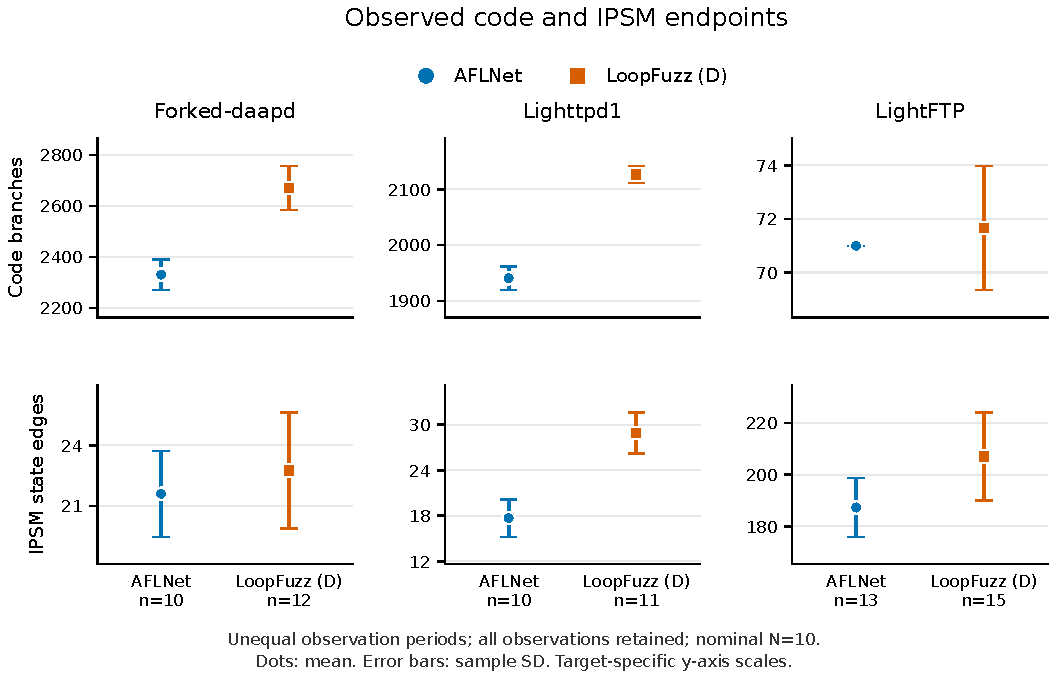
\includegraphics[width=0.92\textwidth]{native_endpoints.pdf}
\caption{A/D code-branch and IPSM state-edge endpoints (mean $\pm$ SD; actual $n$).}
\label{fig:mismatch}
\end{figure*}

The desired controller must accommodate both overestimation and underestimation. Rejecting every state-only candidate could lose useful bridges; promoting every such candidate would treat an imperfect proxy as sufficient evidence for permanent resource allocation. A provisional queue expresses the intermediate conclusion that an input deserves limited descendant validation while its longer-term value remains unproven.

The scope is textual or semi-textual request-response protocols with usable parsers, response extractors, and code feedback. Response-visible state extraction avoids a target-specific internal-state adapter, but the complete controller remains greybox because productivity requires code feedback. It is not a pure black-box system. Encrypted or opaque binary protocols require suitable construction, response, and code-observation adapters before evaluation.

\section{Related Work and Novelty Boundary}
Stateful greybox fuzzing studies how to expose, infer, and schedule protocol state~\cite{aflnet,stateafl,nsfuzz,sgf_usenix22}. AFLNet supplies a response-derived IPSM; StateAFL uses memory snapshots, and NSFuzz traces program state variables. The subsequent AFLNet study revisits coverage-guided protocol fuzzing~\cite{aflnet5years2025}, while greybox protocol-state learning investigates how internal observations inform inferred models~\cite{stateinspector2022}. LoopFuzz retains the response-visible interface and studies its instrumental reliability under an independent code-progress criterion. It does not claim to originate state inference or to first identify misleading responses.

Execution control and feedback interpretation address complementary problems. Nyx-Net uses incremental snapshots for network fuzzing~\cite{nyxnet2022}; SnapFuzz targets high-throughput execution of network applications~\cite{snapfuzz2022}; fault-injection-based network fuzzing provides another approach to exercising protocol interactions~\cite{fuzztructionnet2024}. BLuEMan simulates interactions between actual Bluetooth Low Energy (BLE) stacks~\cite{blueman2025}. DistFuzz combines events, faults, and timing with message-sequence feedback and symmetry-based pruning for distributed systems~\cite{distfuzz2025}. These studies motivate treating execution conditions and observable feedback as separate design choices. Their protocol domains and execution mechanisms are not evidence that LoopFuzz generalizes beyond its evaluated servers.

Structured generation reduces the difficulty of producing admissible inputs. Gramatron generates inputs through grammar automata~\cite{gramatron_effective_grammar_aware_2021}; CarpetFuzz extracts option constraints from documentation~\cite{carpetfuzz_documentation_2023}. FormatFuzzer derives parsers, mutators, and generators from binary-format specifications~\cite{formatfuzzer}; Fuzztruction instead injects faults into a generating program to retain implicit format knowledge~\cite{fuzztruction2023}. MINER uses valid sequence templates and learned request parameters to guide later requests~\cite{miner2023}. These approaches concern how candidates are constructed. Our admission rule asks a subsequent question: whether a candidate has enough independently observed code value to acquire durable queue resources.

ChatAFL uses LLMs for protocol-message generation~\cite{chatafl}; LLMIF derives device-testing inputs from protocol specifications~\cite{llmif_augmented_large_language_2024}; Fuzz4All generates and mutates program inputs across languages~\cite{fuzz4all_universal_fuzzing_large_2024}. FuzzGPT studies unusual programs for deep-learning libraries~\cite{fuzzgpt2024}, and WhiteFox uses compiler source information to guide optimization-triggering tests~\cite{whitefox2024}. ProphetFuzz predicts high-risk option combinations from documentation~\cite{prophetfuzz2024}. Recent studies also address LLM-assisted hybrid fuzzing~\cite{hybridllm2026} and LLM-assisted directed greybox fuzzing~\cite{hgfuzzer2026}. These varied generation objectives reinforce the distinction between a model's proposal and evidence obtained by executing it. The comparison specified here preserves ChatAFL's scheduling lineage. Admission and calibration require separate controlled contrasts.

Adaptive resource allocation is established in fuzzing. The Bandit's States models protocol-state selection as a bandit problem~\cite{bandits_states2023}. T-Scheduler combines Beta--Bernoulli estimation with Thompson sampling for seed scheduling~\cite{tscheduler2024}. Entropic allocates seed energy using estimated information gain~\cite{entropic2020}. SeqFuzzSDN infers extended finite-state machines and plans control-message sequences for software-defined networking controllers~\cite{seqfuzzsdn2026}. These works delimit the contribution. FOX formulates coverage-guided fuzzing as online stochastic control~\cite{fox2024}, while FISHFUZZ dynamically prioritizes targets and seeds using distance information~\cite{fishfuzz2023}. WingMuzz schedules open-source protocol implementations and their seeds to guide blackbox testing~\cite{wingmuzz2025}. Thus neither adaptive selection nor a productivity score is novel by itself. The distinction here is the combination of a response-derived proxy, an independent code-progress target, provisional and durable LLM-candidate admission, and traceable episode-level evidence.

Protocol correctness also requires an oracle beyond apparent acceptance. ProtocolGuard combines specification-derived checks with dynamic verification of non-compliance~\cite{protocolguard2026}; BSFuzzer uses context-aware semantic testing for BLE logic flaws~\cite{bsfuzzer2026}; MerCuriuzz targets logical vulnerabilities in QUIC implementations~\cite{mercuriuzz2026}. These studies examine semantic violations, whereas the proposed calibration reward targets code productivity. A response-state transition or positive code reward therefore does not certify security impact. Magma's ground-truth bug conditions motivate distinguishing bug-related reachability from triggering~\cite{magma2020}; our historical vulnerability protocol additionally requires patch validation and controlled information exposure.

Evaluation methodology is a further boundary. ProFuzzBench and FuzzBench provide structured evaluation settings for protocol and general-purpose fuzzers~\cite{profuzzbench_benchmark_stateful_protocol_2021,fuzzbench2021}. Reliability analyses and prudent evaluation practices require care when interpreting coverage, repeated trials, and resource controls~\cite{reliability_benchmarking_2022,sok_prudent_evaluation_practices_2024}. Our protocol adopts these concerns while keeping available retrospective observations distinct from the unfinished confirmatory comparisons. Candidate-level, episode-level, and controlled rediscovery measurements remain necessary to establish the proposed mechanisms.

\begin{table*}[!tbp]
\centering\small
\caption{Prior mechanisms and novelty boundaries.}
\label{tab:novelty}
\begin{tabularx}{\textwidth}{l Y Y}
\toprule
Prior work & Established focus & Present boundary \\
\midrule
AFLNet; StateAFL; NSFuzz & Response-derived or internal-state feedback. & Proxy calibration, not semantic-state recovery. \\
ChatAFL; LLM synthesis & Protocol-guided message/sequence generation. & Execute-before-promote; bounded provisional validation. \\
The Bandit's States~\cite{bandits_states2023} & Bandit-based protocol-state selection. & Couple proxy calibration with admission. \\
T-Scheduler~\cite{tscheduler2024}; Entropic~\cite{entropic2020} & Posterior- or entropy-based seed scheduling. & Calibrate response proxies. \\
SeqFuzzSDN~\cite{seqfuzzsdn2026} & Learned state models; message-sequence planning. & Response-proxy productivity; candidate admission. \\
Magma~\cite{magma2020}; evaluation studies & Ground-truth bug oracles; repeated trials. & Information-controlled network rediscovery; minimal security-patch pairs. \\
\bottomrule
\end{tabularx}
\end{table*}

\section{Evidence-Calibrated Controller}
\label{sec:design}
This section defines the admission and calibration criteria. Section~\ref{sec:implementation} examines whether the available evidence establishes that these criteria were satisfied. A formal decision rule alone does not demonstrate experimental adherence.

\subsection{LLM proposal interface}
The model receives permitted RFC fragments, seed traces, and observed interaction summaries and returns candidate requests or bounded scheduling hints. Each candidate has a persistent identifier, source state, intended target/frontier, and links to its prompt and raw reply. Message-field hypotheses remain proposals rather than verified protocol grammars.

The information policy excludes CVE identifiers, security advisories, exploit inputs, and patch contents. It specifies the documentation and observed responses available to the model. Adaptive campaigns may produce different prompts despite identical information policies; prompts and responses must therefore remain traceable.

Outputs that propose requests pass through admission. Outputs that only guide scheduling require structural, state-consistency, and seed-consistency checks and cannot insert durable inputs. Parsing or transport failure does not create a positive admission decision. All attempts, retries, failures, and successful replies enter the declared call/token accounting.

\subsection{Admission predicates and evidence separation}
For candidate $x$, $P(x)$ checks the prescribed format, message structure, required fields, lengths, and terminators before execution. A bounded trial then evaluates response acceptability $U(x)$ and reachability $R(x)$: arrival at a declared target/frontier or escape from a recorded rejection sink. \namedref{Table}{tab:predicates} gives observable evidence and decision criteria.

HTTP/FTP 4xx/5xx classes are rejection priors, not a universal semantic definition. An adapter must specify exceptions before a run and retain the response and reason code. Timeout, reset, disconnect, or an unparseable response gives no positive $U$ evidence. A valid response alone is insufficient for $R$. Evidence of security violations is retained independently even when normal request admission fails.

Gain is split into
\begin{align}
\gcode(x)&=\mathbf{1}\{\text{new code coverage or a favored}\nonumber\\
&\hspace{18mm}\text{code-coverage entry}\},\label{eq:gcode}\\
\gstate(x)&=\mathbf{1}\{\text{new IPSM node, state edge, or path}\}.\label{eq:gstate}
\end{align}
Favored status must be grounded in code coverage; merely being queued or state-novel does not qualify. Source-level code branches are the main evaluation surface. If runtime instrumentation observes code edges instead, that reward definition must be prespecified and reported separately. Hit-count novelty is a separate sensitivity condition. Pre-trial coverage and IPSM snapshots establish which gains are new.

\begin{table*}[!tbp]
\centering\small
\caption{Admission predicates and required evidence.}
\label{tab:predicates}
\begin{tabularx}{\textwidth}{l Y Y Y}
\toprule
Predicate & Pass condition & Failure & Measurements \\
\midrule
$P$ & Valid required structure. & Missing fields; invalid lengths/delimiters. & Candidate; criteria; reason; hypothesis version. \\
$U$ & Accepted response. & Rejection; timeout/reset/drop; unparseable reply. & Response; acceptance rule; failure/exception. \\
$R$ & Target/frontier reached or sink escaped. & Sink retained; destination missed. & Source/target; observed state sequence. \\
$\gcode$ & New code coverage or code-supported favored entry. & IPSM-only novelty. & Pre/post coverage; novelty; favored reason. \\
$\gstate$ & New IPSM node, state edge, or path. & Known IPSM structure. & Pre/post IPSM; new state transitions. \\
\bottomrule
\end{tabularx}
\end{table*}

\subsection{Provisional and durable queues}
Let $Q_{\mathrm{prov}}$ contain temporary candidates and $Q_{\mathrm{dur}}$ contain long-term mutation seeds. \namedref{Figure}{fig:architecture} summarizes the three admission outcomes:
\begin{equation}
D(x)=
\begin{cases}
\mathrm{durable}, & P\land U\land R\land\gcode,\\
\mathrm{provisional}, & P\land U\land R\land\neg\gcode\land\gstate,\\
\mathrm{reject}, & \text{otherwise}.
\end{cases}\label{eq:admission}
\end{equation}
IPSM novelty alone is never sufficient for durable promotion. These logical conditions do not assume statistical independence among predicates.

A provisional entry receives at most $H=64$ descendant executions and a local validation deadline of 30 seconds, whichever is exhausted first; the proposed live provisional capacity is 64. These initial settings are checked in the pilot and prespecified before formal runs. Budget checks occur before each descendant execution. Exhaustion expires the entry from active scheduling while preserving the observations supporting that decision. Campaign termination before the validation horizon is censoring, not unproductive expiration.

A descendant supplying qualifying code evidence permits promotion of the replayable parent sequence and productive descendant, subject to the same structural, response, and reachability checks. The record identifies the first productive descendant and the candidate whose status changes. A global code-discovery event is credited once through execution/lineage IDs, not repeatedly to multiple ancestors.

Productivity estimates select where to propose and continue exploration; they do not independently relax Equation~\ref{eq:admission}. Fixed and calibrated arms use identical admission rules and provisional budgets. Calibration thus affects admission outcomes indirectly through exploration opportunities, preserving the causal scheduling comparison.

\begin{figure*}[!tbp]
\centering
\begin{tikzpicture}[
  font=\fontsize{9}{11}\selectfont,
  box/.style={draw=black!75,line width=0.6pt,rounded corners=2pt,
    align=center,text width=23mm,minimum width=26mm,
    minimum height=13mm,inner sep=3pt},
  flow/.style={-{Latex[length=2.5mm,width=1.7mm]},
    draw=black!85,line width=0.85pt,rounded corners=2pt,
    shorten <=1pt,shorten >=1pt},
  failure/.style={flow,draw=black!65,line width=0.7pt,dash pattern=on 3pt off 2pt},
  failbranch/.style={draw=black!65,line width=0.7pt,dash pattern=on 3pt off 2pt},
  condition/.style={font=\fontsize{8.5}{10}\selectfont,
    text=black,fill=white,inner sep=1.2pt,align=center}]
\node[box,fill=blue!5] (llm) at (0,2.8) {LLM\\proposal};
\node[box] (p) at (4.4,2.8) {Structural\\check $P$};
\node[box] (trial) at (8.8,2.8) {Bounded trial\\check $U,R$};
\node[box,fill=blue!5] (gain) at (13.2,2.8) {Separate\\$\gcode,\gstate$};
\node[box,fill=black!4] (rej) at (0,0) {Reject / expire\\retain evidence};
\node[box,fill=orange!12] (prov) at (4.4,0) {Provisional\\queue};
\node[box,fill=orange!5] (validation) at (8.8,0) {Descendant\\validation};
\node[box,fill=blue!8] (dur) at (13.2,0) {Durable\\queue};

\draw[flow] (llm.east)--(p.west);
\draw[flow] (p.east)--node[condition,above] (p_ok) {pass}(trial.west);
\draw[flow] (trial.east)--node[condition,above] (ur_ok) {pass}(gain.west);
\draw[flow] (gain.south)--node[condition,right] (code_gate) {$\gcode$}(dur.north);
\draw[flow] ([xshift=-7mm]gain.south)--(12.5,1.4)--
  node[condition,above] (state_gate) {$\gstate$ only}(4.4,1.4)--(prov.north);
\draw[flow] (prov.east)--(validation.west);
\draw[flow] (validation.east)--node[condition,below] (promotion) {Validated\\code gain}(dur.west);

\coordinate (p_reject) at (4.4,4.2);
\coordinate (trial_reject) at (8.8,4.2);
\coordinate (gain_reject) at (13.2,4.2);
\draw[failure] (gain_reject)--(-2.1,4.2)--(-2.1,0)--(rej.west);
\draw[failbranch] (p.north)--node[condition,right] (p_fail) {$\neg P$}(p_reject);
\draw[failbranch] (trial.north)--node[condition,right] (ur_fail) {$\neg U\lor\neg R$}(trial_reject);
\draw[failbranch] (gain.north)--node[condition,left] (no_gain) {Neither gain}(gain_reject);
\fill[black!65] (p_reject) circle[radius=1pt];
\fill[black!65] (trial_reject) circle[radius=1pt];
\draw[failure] (validation.south)--(8.8,-1.35)--
  node[condition,above] (expiry) {Budget exhausted}(0,-1.35)--(rej.south);
\end{tikzpicture}
\caption{Evidence-gated admission and two-tier queues.}
\label{fig:architecture}
\end{figure*}

\subsection{State-selection episodes and independent reward}
An episode begins when the scheduler selects response-derived state $s$ and a seed capable of reaching it. It receives one fixed execution-energy budget. Individual executions within the episode do not generate repeated posterior updates. Mutation counts, reset failures, elapsed time, and budget exhaustion are measured. Infrastructure-interrupted episodes are incomplete, rather than silently assigned reward zero.

For completed episode $t$ targeting $s_t$, let $\Delta B_t$ count previously unseen code branches discovered within that episode. The main reward is
\begin{equation}
r_t=\mathbf{1}\{\Delta B_t>0\}.
\label{eq:reward}
\end{equation}
A declared code-edge instrumentation variant is admissible, but IPSM novelty is excluded. Favored descendants are a secondary sensitivity reward. Equal energy prevents a state appearing more productive merely because it receives more executions. Trial execution, ordinary mutation, and provisional validation use distinct event types to avoid duplicate updates.

$\theta_s$ denotes the probability of positive code reward conditional on selecting $s$ under the episode policy and current campaign phase. It is instrumental utility, not the probability that $s$ is a true semantic state. $U$ continues to mean response acceptability; utility is never denoted $U(s)$.

\subsection{Discounted productivity estimates}
Each state starts with $\alpha_s=\beta_s=1$ and
\begin{equation}
\theta_s\sim\operatorname{Beta}(\alpha_s,\beta_s),\qquad
\widehat{\theta}_{s,t}^{\,\mathrm{pre}}
=\frac{\alpha_{s,t}}{\alpha_{s,t}+\beta_{s,t}}.
\end{equation}
For a completed selected-state episode:
\begin{align}
\alpha_s&\leftarrow1+\gamma(\alpha_s-1)+r_t,\\
\beta_s&\leftarrow1+\gamma(\beta_s-1)+(1-r_t).
\label{eq:update}
\end{align}
The proposed discount is $\gamma=0.995$, with sensitivity values $\{0.99,0.995,1.0\}$. Parameters are prespecified after the pilot and before inspecting formal results. At $\gamma=1$, updates reduce to cumulative Beta--Bernoulli counts. For $\gamma<1$, excess prior counts are discounted to respond to changing productivity as coverage saturates.

The term productivity posterior denotes this discounted working model. With discounting it is not the exact posterior of a stationary Bernoulli process. Discounting occurs on completed episodes for the selected state; unselected states do not automatically age in wall-clock time. The update clock and cold start are therefore explicit applicability limits.

Every calibration metric uses the pre-update mean recorded before reward. Post-update predictions would leak the outcome into their own evaluation. Thompson samples are recorded separately and are not substituted for predicted Bernoulli probabilities in reliability calculations.

\subsection{Calibrated scheduling}
The topology term favors underexplored observed states:
\begin{equation}
F(s)=
\begin{cases}
4,&s\text{ is newly reachable or }\deg^+(s)\leq1,\\
2,&1<\deg^+(s)\leq3,\\
1,&\deg^+(s)>3.
\end{cases}
\end{equation}
Only reachable states with eligible seeds participate. $\deg^+(s)$ counts outgoing IPSM state edges, not code branches. Let $B(s)$ denote the inherited base weight shared by C, D, and E. Define
\begin{equation}
\operatorname{Frontier}(s)=B(s)F(s).
\end{equation}
Keeping this factor and any warm-up policy fixed prevents calibration from simultaneously changing the baseline scheduler. Adapting posterior-guided randomization~\cite{thompson1933} to the discounted, frontier-weighted controller, draw
\begin{equation}
\widetilde{\theta}_s\sim\operatorname{Beta}(\alpha_s,\beta_s)
\end{equation}
and calculate
\begin{equation}
S(s)=\operatorname{Frontier}(s)[\epsilon+(1-\epsilon)\widetilde{\theta}_s],
\qquad\epsilon=0.1.
\label{eq:score}
\end{equation}
Select a state with probability proportional to $S(s)$, recording the pseudorandom seed. This is Thompson-sampled weighted selection, not an argmax policy. Under a finite eligible set, the positive floor gives nonzero selection probability, not a fixed number of selections.

The fixed-policy comparator retains the original penalty:
\begin{equation}
S_D(s)=\operatorname{Frontier}(s)\rho_{\mathrm{fixed}}(s).
\end{equation}
Its cached queue-yield ratio $p_s=D_s/(N_s+1)$ counts interesting queued paths $D_s$ per state selections $N_s$. It is not a calibrated Bernoulli probability and can reflect state-only novelty or unequal execution energy. E replaces only $\rho_{\mathrm{fixed}}$ with the calibrated factor in Equation~\ref{eq:score}, preserving the shared base, admission, prompts, triggers, repair settings, and caps. Integer score conversion and the initial round-robin schedule must be prespecified and verified before comparison.

\begin{figure}[!tbp]
\centering
\begin{tikzpicture}[>=Latex,font=\small,
box/.style={draw,rounded corners,align=center,text width=61mm,minimum height=9mm},
arr/.style={->,thick}]
\node[box] (pre) {Pre-update mean; Thompson sample};
\node[box,below=5mm of pre] (run) {Select state; fixed-energy episode};
\node[box,below=5mm of run] (reward) {Independent code reward};
\node[box,below=5mm of reward] (update) {Discounted posterior update};
\draw[arr](pre)--(run);\draw[arr](run)--(reward);\draw[arr](reward)--(update);
\end{tikzpicture}
\caption{Online calibration from pre-update predictions and independent code rewards.}
\label{fig:posterior}
\end{figure}

\begin{algorithm}[t]
\small\caption{Evidence-gated candidate processing}\label{alg:admission}
\DontPrintSemicolon
\KwIn{Candidate $x$, target, fixed pre-trial state}
Record candidate, prompt, reply, and lineage identifiers\;
\If{$\neg P(x)$}{Record structural rejection; stop processing $x$\;}
Execute one bounded trial without durable queue insertion\;
Record $U,R,\gcode,\gstate$ and reason codes\;
\If{$P\land U\land R\land\gcode$}{Promote $x$ to $Q_{\mathrm{dur}}$\;}
\ElseIf{$P\land U\land R\land\neg\gcode\land\gstate$}{
Insert $x$ into $Q_{\mathrm{prov}}$\;
\While{budget, validation deadline, and campaign time remain}{
Check budget before the next descendant execution\;
Execute and record one descendant\;
\If{qualifying code gain and validation pass}{
Record first productive descendant; promote; end validation\;
}
}
Record expiration or campaign censoring if still provisional\;
}
\Else{Record rejection\;}
Preserve security-oracle evidence separately\;
\end{algorithm}

\subsection{Intervention policy and optional repair}
Plateau interventions follow prespecified detection, timing, and retry rules. The baseline trigger combines IPSM state-edge growth with a sequence of unproductive selections. This dependence on the state proxy is held constant across the causal comparisons; scheduling calibration does not itself validate the intervention trigger.

The confirmatory C/D/E design requires repair to be disabled. Counterexample-guided repair is an optional feature without quantitative evaluation in this study. The available observations do not verify repair status in every run, and no effectiveness or cost benefit is attributed to it.


\section{Operational Validity and Measurement}
\label{sec:implementation}
The evaluated system can represent code and state novelty separately, provisionally retain candidates, and condition state selection on productivity estimates. The available observations do not establish that these mechanisms operated as specified in every trial. Operational validity therefore depends on both effective experimental conditions and the sequence of admission decisions.

Candidate retention may precede behavioral verification. A subsequent $U/R$ failure need not reverse that decision, so strict adherence to Equation~\ref{eq:admission} is not established. Coverage-based retention may also reflect execution-frequency changes rather than newly covered code branches. Similarly, evaluating provisional budgets only after an entire mutation cycle can exceed the prescribed limits.

IPSM novelty is assessed after changes associated with candidate retention. A candidate without prior code-based retention may therefore lack an independent state-only novelty assessment. This dependency can suppress the provisional condition by construction. An absence of provisional observations cannot distinguish effective filtering from a missing opportunity for provisional validation.

The available $P$ decisions can reflect structural recognition without establishing full request validity. Likewise, $R$ may indicate a state transition without confirming arrival at the intended target or frontier. These observations are weaker than the proposed predicates. \namedref{Table}{tab:implementation} summarizes the resulting threats to operational validity.

\begin{table*}[!tbp]
\centering\small
\caption{Operational criteria and evidence limitations.}
\label{tab:implementation}
\begin{tabularx}{\textwidth}{Y Y Y}
\toprule
Requirement & Current boundary & Evaluation consequence \\
\midrule
Gate before promotion & Retention may precede $U/R$. & Queue protection unverified. \\
Independent state-only evidence & State assessment follows retention. & Zero provisional counts may be structural. \\
Complete $P/R$ verification & $P$: recognition; $R$: transition. & Validity and reachability unverified. \\
New-code reward & Execution-frequency novelty may contribute. & Distinguish branches, frequency, and retention. \\
Fixed-energy episodes & Variable energy; zero executions. & Unequal opportunities. \\
Strict provisional budget & Post-round budget checks. & 64-mutation/30-second limits may be exceeded. \\
Verified run conditions & Initial and effective settings may differ. & Verify conditions throughout each run. \\
Total call/token caps & 64-call cap: plateau only; tokens unverified. & Total-budget fairness unverified. \\
Repair off in C/D/E & Repair status incompletely verified. & Arm labels do not prove adherence. \\
\bottomrule
\end{tabularx}
\end{table*}

\subsection{Measurement structure and traceability}
The measurement framework distinguishes experimental conditions, candidate generation, admission trials, provisional outcomes, scheduling episodes, and security outcomes; optional repair adds a seventh observation class. \namedref{Table}{tab:events} specifies the corresponding evidence. Each observation retains its trial identity, measurement-definition version, temporal order, and time. CVE identities remain isolated benchmark metadata. Missing observations are not assigned zero values. Conditions distinguish target/fuzzer and model/service versions, sampling parameters, random seeds, and CPU/memory limits. Admission measurements retain reasons, state sequences, and separate pre/post code and IPSM counts. Episodes retain pre/post $\alpha,\beta$, the pre-update mean, Thompson sample, and frontier/selection scores.

\begin{table*}[!tbp]
\centering\footnotesize
\caption{Observation classes and required measurements.}
\label{tab:events}
\begin{tabularx}{\textwidth}{@{}>{\raggedright\arraybackslash}p{0.27\textwidth} Y Y@{}}
\toprule
Observation class & Experimental context & Measurements / outcomes \\
\midrule
Experimental conditions & Arm; software/model versions; environment; sampling seed. & Call/token caps; resources; period; termination. \\
Candidate generation & Candidate/prompt; lineage; request/response; action; source/target. & Input/output tokens; generation time. \\
Admission trial & Candidate/trial; $P/U/R$; responses; reachability. & Code/IPSM changes; priority; latency; decision. \\
Provisional validation & Candidate; budget; first productive descendant. & Executions; code gain; conversion/expiration; latency; censoring. \\
State-selection episode & State/seed; pre-update posterior; sample; selection scores. & Mutations; code/IPSM gain; reward; updated posterior; duration/completion. \\
Security outcome & Anonymous oracle; reproducer; diagnostics; root cause. & Reached/triggered; first trigger; version-pair outcomes. \\
Repair (optional) & Lineage; counterexample; hypotheses; changed component. & Validation; post-repair predicates/gain; tokens; latency. \\
\bottomrule
\end{tabularx}
\end{table*}

Confirmatory evaluation requires at least 99.9\% completeness of candidate observations, an identifiable candidate for every trial, an identifiable episode for every posterior update, and reconstructable promotion decisions. The denominator includes unsuccessful generation and interpretation attempts. Observation availability, correspondence across measurements, and agreement between reported decisions and actual queue membership are assessed separately.

\section{Evaluation Scope and Validation Criteria}
\label{sec:protocol}
The present study is a retrospective, descriptive analysis of benchmark, ablation, and vulnerability-replay observations. The five-arm design and measurement definitions below state the conditions required for causal validation; they do not establish that a matched confirmatory evaluation was completed. Prior registration, prospective parameter selection, and completed pilot validation cannot be inferred from these records.

\subsection{Research questions}
\begin{enumerate}
\item \textbf{RQ1: State/code alignment.} How reliably does response-derived state novelty predict downstream code progress across targets and campaign phases? Measure IPSM state-edge/code-branch alignment, episode productivity, calibration, and boundary cases.
\item \textbf{RQ2: Admission.} Does execute-before-promote reduce durable queue pollution and improve downstream productivity under matched proposal and scheduling conditions? Compare D with C.
\item \textbf{RQ3: Calibration.} Does online productivity calibration improve scheduling over a fixed response-state heuristic? Compare E with D.
\item \textbf{RQ4: Historical vulnerability rediscovery.} Does the controller improve reproducible rediscovery under independent reached/triggered oracles and patch validation?
\item \textbf{RQ5: Cost and applicability.} What runtime, throughput, and LLM costs arise, and under which target characteristics does the method fail to help?
\end{enumerate}
The directional hypotheses are improved downstream productivity for D over C and greater area under the code-branch coverage curve (AUC) for E over D. Regressions, null results, and uncertainty are reported per target rather than hidden in pooled means or replaced by increased IPSM state-edge counts.

\subsection{Five arms and causal comparisons}
\begin{table*}[!tbp]
\centering\small
\caption{Required configurations for arms A--E.}
\label{tab:arms}
\begin{tabularx}{\textwidth}{l c Y Y Y}
\toprule
Arm & LLM & Admission & Scheduler & Role \\
\midrule
A: AFLNet & No & Original AFLNet & AFLNet & Non-LLM baseline. \\
B: Controlled ChatAFL & Yes & ChatAFL direct/open-loop & ChatAFL lineage & B--A: LLM-lineage comparison. \\
C: LoopFuzz-direct & Yes & Parseable to durable & Fixed LoopFuzz & Admission counterfactual. \\
D: LoopFuzz-gated-fixed & Yes & Evidence gate; provisional queue & Same fixed LoopFuzz & D--C: admission effect. \\
E: LoopFuzz-gated-calibrated & Yes & Identical to D & Productivity calibration & E--D: calibration effect. \\
\bottomrule
\end{tabularx}
\end{table*}

C/D share model configuration, prompt construction, trigger, repair setting, scheduler, and budget policy; the intended intervention is admission. E/D share admission and differ only in state selection. Controlled ChatAFL retains its scheduling lineage; replacing it with the LoopFuzz scheduler would change the baseline. B--A is not an isolated admission comparison.

Proposal control has two scopes. Paired diagnostics evaluate the same candidate under direct and gated admission from an identical initial target and campaign state, with equal descendant budgets. This comparison supports a candidate-level counterfactual. Independent adaptive campaigns diverge, so equal policies do not guarantee identical prompts or model outputs. Replay can assess structural validation and admission decisions under matched initial conditions, but cannot establish equivalence to an independently evolving campaign.

\subsection{Targets and experimental controls}
The primary design contains nine servers: four FTP servers, Exim (SMTP), Live555 (RTSP), Kamailio (SIP), Forked-daapd (DAAP/DACP over HTTP), and Lighttpd1 (HTTP). \namedref{Table}{tab:targets} identifies the target protocols and experimental conditions. Source revisions are fixed by the benchmark configuration; endpoints and initialization procedures follow the recorded trial conditions. Build identity beyond those revisions remains unverified. In the table, yes/no denotes dictionary use, and unrecorded means that no reset procedure was recorded; it does not establish that state restoration occurred.

\begin{table*}[!tbp]
\centering\small
\caption{Target protocols and recorded test conditions.}
\label{tab:targets}
\begin{tabular*}{\textwidth}{@{\extracolsep{\fill}}lllllcl@{}}
\toprule
Target & Protocol & Source revision & Endpoint (localhost) & Seed protocol & Dictionary & Reset \\
\midrule
LightFTP & FTP & 139af7c & tcp/2200 & FTP & yes & cleanup \\
bftpd & FTP & 6.1 release & tcp/21 & FTP & yes & cleanup \\
ProFTPD & FTP & 61e621e743346 & tcp/21 & FTP & yes & cleanup \\
Pure-FTPd & FTP & 10122d9f & tcp/21 & FTP & yes & cleanup \\
Exim & SMTP & d6a5a05b84 & tcp/25 & SMTP & yes & cleanup \\
Live555 & RTSP & live.2023.05.10 & tcp/8554 & RTSP & yes & unrecorded \\
Kamailio & SIP & a2209018fb03d & udp/5060 & SIP & no & PJSIP routine \\
Forked-daapd & DAAP/DACP & 2ca10d9 & tcp/3689 & DAAP & no & unrecorded \\
Lighttpd1 & HTTP & 9f38b63cae3e2 & tcp/8080 & HTTP & yes & unrecorded \\
\bottomrule
\end{tabular*}
\end{table*}

Each run executes in its own Docker container with loopback-only networking and an AFL-instrumented build of the pinned revision; the recorded invocation fixes the seed corpus, dictionary, endpoint, and per-execution reset script listed in \namedref{Table}{tab:targets}. Dockerfile pins document the built revision but are not themselves embedded in the per-run evidence, and \texttt{latest} image tags do not record rebuild provenance.

Each causal comparison requires identical software versions, compilation settings, coverage instrumentation, seeds, replay procedures, and reset policies. Trial order is randomized within machine blocks and balanced across machines and time periods. Random seeds, resource allocations, measured CPU consumption, resource contention, and execution rates characterize each trial. Allocated resources do not establish equal consumption; initialization, model waiting, validation, mutation, and termination all contribute to experimental cost. Resource-efficient benchmarking also makes the cost of obtaining reliable comparisons an explicit concern~\cite{greenbenchmark2023}. The proposed analysis therefore distinguishes allocated CPU-hours, measured consumption, and actual search exposure.

Each arm initially receives 10 independent 24-hour runs per target; C/D/E receive 10 more, reaching 20 each. For nine targets and one allocated CPU per run, the stages require 10,800 and 6,480 CPU-hours, totaling 17,280 before overhead/failures. These are planned resources, not measured usage. A four-target pilot covers Forked-daapd, Lighttpd1, LightFTP, and ProFTPD or Pure-FTPd with five arms, three runs, and four to six hours each. Pilot observations are excluded from formal inference.

An intention-to-run analysis accounts for every planned and initiated trial, including completion, timeout, target or fuzzer failure, infrastructure or measurement failure, exclusion, and repetition, with reasons linking repeated attempts. Low coverage never justifies exclusion. Only prespecified infrastructure failures permit repetition. Interrupted observations are not extended to 24 hours; they contribute failure or censoring outcomes according to the estimand, with sensitivity analysis. Restriction to completed trials does not constitute intention-to-run analysis.

\subsection{LLM fairness and configuration}
The confirmatory design requires equal policies and resource ceilings across LLM arms; actual calls and token usage may differ with adaptive trajectories. In \namedref{Table}{tab:llm}, configuration values are supported by final observations for C/D/E and the sensitivity groups, while equivalent B observations are unavailable. Timeout, retry, seed, and template descriptions are source-derived; they do not independently verify the settings of every executed build. Unresolved settings remain identified explicitly.

\begin{table*}[!tbp]
\centering\small
\caption{LLM settings for C/D/E and sensitivity groups; B unverified.}
\label{tab:llm}
\begin{tabularx}{\textwidth}{Y >{\centering\arraybackslash}Y Y}
\toprule
Parameter & Recorded value & Comparison requirement \\
\midrule
Model / version / service & codex-auto-review; cctq.ai & Same resolved version; name insufficient. \\
Temperature by call class & grammar 0.5; plateau 1.2 & Match each call class. \\
Top-$p$ / presence/frequency penalties & top-$p$ 1.0; penalties unrecorded & Explicit values or defaults. \\
Output tokens per attempt & 4,096 & Same cap; include truncation/failures. \\
Attempted-call / total-token caps & call cap 64; token cap 0 (unset) & Count all classes and retries. \\
Timeout / retry policy & 120\,s request, 30\,s connect, 60\,s low-speed abort; 2--5 retries by call class, 2\,s apart; fatal provider errors abort retries & Same policy; include waits/failures. \\
Model seed / support & none; no seed parameter is sent & Document support; determinism unassured. \\
Prompt corpus / template & no version identifier; per-request prompt hashes logged; template identity tracks the fuzzer commit & Same information policy; traceable exchanges. \\
Plateau cadence / threshold / reset & state-edge threshold 512; cadence unrecorded & Same intervention/state-growth criteria. \\
\bottomrule
\end{tabularx}
\end{table*}

An output-token limit per request is distinct from a total campaign limit. A recorded token-limit value of zero does not establish equal-token control without evidence of the effective policy. Monetary costs require verifiable usage and applicable prices; unavailable costs remain unspecified.

The present cost analysis reports observed calls and tokens descriptively. Estimating code gain per candidate, per 1,000 total tokens, or at matched cumulative budgets would additionally require linked gain and complete usage measurements. These efficiency effects are not estimated here. Future comparisons must account for unsuccessful requests, retries, validation, and any repair costs; zero-denominator ratios remain undefined.

\subsection{Mechanism and calibration metrics}
Available results comprise recorded candidate and trial counts, first-failure distributions, disposition labels, trial latency, and exploratory episode diagnostics. Denominators accompany reported rates. The following descendant-based criteria define what would be required to validate admission quality; they are not measured outcomes of this study.

For a prospective evaluation, downstream productivity uses a fixed descendant horizon rather than admission gain. For a declared cohort $\mathcal{C}$ of $N$ candidates enrolled before their outcomes are known, let $Y_i(H)=1$ if a later descendant produces new code coverage within $H$ executions, and $0$ if the full horizon is observed without gain. With complete observation, define
\begin{equation}
\operatorname{Productivity@}H=\frac{1}{N}\sum_{i\in\mathcal{C}}Y_i(H).
\end{equation}
The proposed initial horizon is $H=64$; no such outcome is estimated here. The admission trial is excluded. A positive outcome can be established early; a negative requires the complete horizon. With $n_+$ known positives and $n_?$ censored unresolved candidates, cohort bounds are $[n_+/N,(n_++n_?)/N]$. A valid paired diagnostic would reserve the same full validation horizon for both controllers and retain incomplete observations in the denominator. Durable and provisional cohorts are distinct; post-promotion productivity requires a fresh horizon.

An avoided-pollution claim requires a paired C--D comparison: direct-arm durable candidates without downstream gain must be linked to their retention under gating. D-arm rejections alone do not establish avoided pollution. Estimating false negatives would require a predeclared random sample of rejected candidates, common initial conditions, descendant lineage, and recorded validation costs. These measurements are unavailable in the present study.

For complete episodes, $p_t=\widehat{\theta}_{s_t,t}^{\,\mathrm{pre}}$ predicts later reward $r_t$. We assess probabilistic accuracy with the binary Brier score (BS), also used in software defect prediction~\cite{validation2017}:
\begin{equation}
\mathrm{BS}=\frac{1}{n}\sum_{t=1}^{n}(p_t-r_t)^2.
\end{equation}
We adapt the binned expected calibration error (ECE) of Guo et al.~\cite{guo2017calibration} to binary episode productivity: within ten fixed equal-width bins, we compare the mean predicted reward probability with the observed reward frequency and weight each absolute gap by its episode count. This evaluates event probabilities rather than predicted-class confidence. Bin counts accompany the estimate; empty bins remain unestimated. Reliability plots and precision--recall analysis~\cite{davis2006pr} accompany the BS. We report non-interpolated average precision (AP): precision at each distinct score threshold weighted by its recall increment. This quantity differs from trapezoidal precision--recall area; it is left undefined when there are no positive episodes. Compare the BS to a prequential base-rate predictor because rare rewards can make uninformative near-zero predictions look accurate. IPSM state-edge/code-gain ratios with zero code gain are undefined or shown as separate zero-gain cases.

Episodes within a run are dependent, so inferential uncertainty requires run-level clustering and target-specific analysis. Posterior trajectories and state weights remain descriptive diagnostics. A state/code association would require linked measurements within target and phase; pooled counts across unlike programs cannot establish that relationship.

\subsection{Coverage and statistical analysis}
Primary coverage outcomes are code-branch AUC over 24 hours and final code-branch count. AUC uses each run's cumulative time series with a common interpolation convention and instrumentation, in branch-hours. Endpoints recorded at unequal durations are not substituted. Time to 95\% of a target-specific common reference endpoint uses a threshold prespecified before formal comparisons; unreached thresholds are censored.

Per target, report mean, median and dispersion. Bootstrap resampling~\cite{efron1979} operates on whole runs; the percentile 95\% confidence intervals (CIs) and resampling hierarchy are analysis choices specified here. For independent run-level contrasts, report two-sided Mann--Whitney U tests~\cite{mann1947} with ties accounted for, and Cliff's $\delta$~\cite{cliff1993}, oriented as $\Pr(X_{\rm treatment}>X_{\rm comparator})-\Pr(X_{\rm treatment}<X_{\rm comparator})$. The rank test is not interpreted as a test of median differences alone. The primary family comprises 36 coverage tests across nine targets: D--C and E--D contrasts for final branches and AUC. Apply the Benjamini--Hochberg procedure~\cite{benjamini1995} at nominal $q=0.05$. Its original guarantee assumes independent test statistics; shared comparator runs and correlated coverage outcomes do not establish that condition here. Report adjusted values without claiming unconditional false-discovery-rate control. A confirmatory admission-mechanism family would contain nine D--C productivity contrasts; these are not estimated here. Other diagnostics and sensitivity tests are exploratory. Effect direction is treatment minus comparator.

Cross-target summaries use equal-weight target effects and a hierarchical bootstrap resampling targets, then runs within targets. Raw branch counts from different programs or individual executions are not pooled as independent samples. Target regressions and uncertainty accompany aggregates. A future historical time-to-trigger analysis would use Kaplan--Meier estimates~\cite{kaplan1958} under non-informative right censoring, alongside CVE-specific deadline recall. Fuzzer-failure interruptions are distinguished because censoring may be informative.


\section{Available Evidence and Results}
\label{sec:results}
The evaluation analyzes recorded outcomes from the benchmark and ablation studies. Results obtained under earlier configurations do not establish the effectiveness of the proposed controller. Result tables contain observed quantities; unmeasured effects are described as evidence limitations and are not assigned zero values.

\subsection{Sample composition and observation periods}
The dataset contains 94 AFLNet (A), 91 ChatAFL (B), 104 benchmark LoopFuzz (D), 90 direct-admission (C), and 91 calibrated (E) observations. The sensitivity conditions contain 81 observations at $\gamma=0.99$ and 91 at $\gamma=1.0$. End-of-run configuration events recorded inside each archive label 17 of the 90 direct-directory observations and 12 of the 91 calibrated-directory observations with the fixed-policy arm; the $\gamma=0.99$ and $\gamma=1.0$ directories contain 15 and 12 such records. For the direct-directory records, the recorded dispositions (all durable, none rejected) corroborate direct admission; the calibrated- and sensitivity-directory records cannot be behaviorally distinguished because posterior-episode logging is active in every LoopFuzz condition. Fuzzer builds also differ within arms: D spans four recorded commits (78/12/9/5 runs), C two (83/7), and E two (71/20), while both sensitivity conditions use a single commit. Counts below retain the directory-level assignment. All available observations are retained without assuming independence. The nominal target is ten trials per condition; actual sample sizes $n$ remain explicit. Means and sample SDs use observed values only, with no imputation for unavailable trials.

All 104 benchmark LoopFuzz D observations are reported as completed; \namedref{Table}{tab:observed_inventory} gives target-specific counts. Termination categories alone do not establish memory exhaustion or vulnerability activation. Reported runtime measures active fuzzing rather than total CPU consumption or the entire experimental period.

The benchmark LoopFuzz observations also constitute the fixed-policy admission condition D and are counted once. The direct-admission and calibrated-scheduling conditions correspond to C and E. Two sensitivity groups use $\gamma=0.99$ and $\gamma=1.0$. The configuration uncertainty in \namedref{Table}{tab:implementation} and unequal sample sizes preclude a fully matched comparison. Recorded posterior estimates alone do not establish a calibration effect.

% Generated from current Key_Experiment archives on 2026-09-30.
\begin{table*}[!tbp]
\centering\small
\caption{Observed trial counts and D-arm status ($N=10$ nominal runs).}
\label{tab:observed_inventory}
\begin{tabular}{lrrrrrl}
\toprule
Target & AFLNet & ChatAFL & LoopFuzz(D) & Completed(D) & Exit 137(D) & Duration (min) \\
\midrule
LightFTP & 13 & 11 & 15 & 15 & 0 & 1473--1522 \\
bftpd & 10 & 10 & 10 & 10 & 0 & 1499--1510 \\
ProFTPD & 10 & 10 & 12 & 12 & 0 & 1489--1518 \\
Pure-FTPd & 11 & 10 & 10 & 10 & 0 & 1460--1472 \\
Exim & 10 & 10 & 10 & 10 & 0 & 1477--1486 \\
Live555 & 10 & 10 & 12 & 12 & 0 & 1489--1505 \\
Kamailio & 10 & 10 & 12 & 12 & 0 & 1472--1518 \\
Forked-daapd & 10 & 10 & 12 & 12 & 0 & 1474--1524 \\
Lighttpd1 & 10 & 10 & 11 & 11 & 0 & 1469--1523 \\
\bottomrule
\end{tabular}
\end{table*}
\begin{table*}[!tbp]
\centering\small
\caption{A/D terminal coverage (mean $\pm$ SD); descriptive comparisons.}
\label{tab:observed_endpoints}
\begin{tabular}{lrrrr}
\toprule
 & \multicolumn{2}{c}{Code branches} & \multicolumn{2}{c}{IPSM state edges} \\
Target & AFLNet & LoopFuzz(D) & AFLNet & LoopFuzz(D) \\
\midrule
LightFTP & 71.0$\pm$0.0 & 71.7$\pm$2.3 & 187.3$\pm$11.3 & 207.0$\pm$17.0 \\
bftpd & 486.0$\pm$8.8 & 502.7$\pm$7.5 & 163.1$\pm$15.4 & 226.7$\pm$14.0 \\
ProFTPD & 5053.8$\pm$97.4 & 5428.1$\pm$104.0 & 190.5$\pm$27.9 & 305.3$\pm$20.3 \\
Pure-FTPd & 1076.4$\pm$89.6 & 1223.3$\pm$29.7 & 236.5$\pm$26.7 & 321.4$\pm$11.1 \\
Exim & 3798.8$\pm$43.3 & 3914.9$\pm$20.9 & 88.8$\pm$5.2 & 152.7$\pm$9.3 \\
Live555 & 2893.6$\pm$14.5 & 3067.1$\pm$29.5 & 96.1$\pm$8.6 & 170.1$\pm$11.1 \\
Kamailio & 10002.6$\pm$144.2 & 10631.2$\pm$472.9 & 109.4$\pm$9.7 & 128.2$\pm$26.6 \\
Forked-daapd & 2330.8$\pm$60.0 & 2670.2$\pm$87.3 & 21.6$\pm$2.1 & 22.8$\pm$2.9 \\
Lighttpd1 & 1940.7$\pm$21.2 & 2126.7$\pm$15.7 & 17.7$\pm$2.5 & 28.9$\pm$2.7 \\
\bottomrule
\end{tabular}
\end{table*}
\begin{table*}[!tbp]
\centering\small
\caption{D-arm candidate and episode counts; dispositions are reported labels.}
\label{tab:observed_log_counts}
\begin{tabular}{lrrrrrr}
\toprule
Target & Candidates & Trials & Reject & Provisional & Durable & Episodes \\
\midrule
LightFTP & 48 & 48 & 44 & 0 & 4 & 13604 \\
bftpd & 13 & 13 & 13 & 0 & 0 & 3249 \\
ProFTPD & 0 & 0 & 0 & 0 & 0 & 2395 \\
Pure-FTPd & 173 & 173 & 166 & 0 & 7 & 5378 \\
Exim & 24 & 24 & 24 & 0 & 0 & 2650 \\
Live555 & 851 & 851 & 844 & 0 & 7 & 7687 \\
Kamailio & 253 & 253 & 249 & 0 & 4 & 9004 \\
Forked-daapd & 412 & 411 & 410 & 0 & 1 & 12056 \\
Lighttpd1 & 453 & 453 & 453 & 0 & 0 & 21570 \\
\bottomrule
\end{tabular}
\end{table*}

The complete target--arm results, including both gamma sensitivity groups, are reported in \ref{sec:archive_appendix} (\namedref{Table}{tab:archive_arms}).

\namedref{Table}{tab:observed_endpoints} includes every available A and D observation. Code-branch and IPSM state-edge endpoints represent the terminal measurements from each trial. For all 642 experimental records, the final trajectory measurement agrees with the corresponding endpoint. These are descriptive observations at unequal durations, rather than matched 24-hour outcomes. Sample SDs describe variation among the available observations; no causal effect or significance claim is attached to the endpoint differences.

\subsection{RQ1: Current alignment observations}
Forked-daapd has mean code-branch endpoints of $2330.8\pm60.0$ for AFLNet and $2670.2\pm87.3$ for LoopFuzz, while IPSM state-edge endpoints are $21.6\pm2.1$ and $22.8\pm2.9$. This direction does not reproduce the older motivating claim of code regression. The difference cannot be attributed to calibration, which is not established as active.

Lighttpd1 increases in both endpoint metrics: code branches from $1940.7\pm21.2$ to $2126.7\pm15.7$, and IPSM state edges from $17.7\pm2.5$ to $28.9\pm2.7$. These aggregate observations do not demonstrate the hypothesized small state expansion with hidden code progress. LightFTP has near-equal code endpoints, $71.0\pm0.0$ versus $71.7\pm2.3$, with larger LoopFuzz IPSM state-edge counts, $187.3\pm11.3$ versus $207.0\pm17.0$. That pattern motivates a saturation analysis but does not establish the full time course or identify individual misleading states.

All three cases require common experimental versions, matched observation periods, and linked state/execution measurements before supporting a mechanism claim. \namedref{Figure}{fig:reliability} instead examines a narrower estimand: agreement between pre-update probabilities and the binary reward associated with coverage-based retention, separately by target. All 32,946 E observations satisfy probability, Beta-mean, binary-response, uniqueness, temporal-order, and within-episode discounted-update consistency checks. Excluding 6,562 episodes with no mutations leaves 26,384 episodes from 91 runs. Three discontinuities between successive posterior estimates are retained; missing history is not reconstructed. These measurements alone do not verify that every run followed the intended scheduling policy.

\namedref{Table}{tab:logged_calibration} reports the BS, ten-bin ECE, and non-interpolated AP; lower BS/ECE is better. Its prequential reference uses only past included same-run rewards with Beta(1,1) smoothing. Percentile 95\% CIs use 2,000 bootstrap resamples of whole runs within each target; they do not resolve unknown dependence between launches. Empty bins have no estimate, and bins represented by fewer than two runs have no CI. In \namedref{Figure}{fig:reliability}, points pair the bin-mean pre-update prediction with reward frequency; the diagonal denotes perfect calibration. Lower strips give positive-mutation episode counts, with actual runs $n$, episodes $m$, and nominal $N=10$. The observed reward reflects coverage-based retention, which may include execution-frequency novelty; positive mutation counts do not establish complete fixed-energy episodes. These diagnostics therefore do not fill independent code-branch calibration outcomes; the equal-energy subset rows in \namedref{Table}{tab:mechanisms} condition the same proxy reward on one fixed energy and inherit these limits.

% Generated logged-reward diagnostics, not fixed-energy source-branch outcomes.
\begin{table*}[t]
\centering\footnotesize
\caption{Proxy-reward calibration in E (95\% CIs in brackets).}
\label{tab:logged_calibration}
\begin{tabularx}{\textwidth}{l r r *{4}{>{\centering\arraybackslash}X}}
\toprule
Target & $n$ & Episodes & BS & Reference BS & ECE (10 bins) & AP \\
\midrule
LightFTP & 10 & 6,622 & \shortstack{0.188\\{[0.178, 0.198]}} & \shortstack{0.183\\{[0.172, 0.195]}} & \shortstack{0.166\\{[0.161, 0.172]}} & \shortstack{0.452\\{[0.430, 0.471]}} \\
bftpd & 10 & 2,643 & \shortstack{0.249\\{[0.243, 0.257]}} & \shortstack{0.247\\{[0.243, 0.252]}} & \shortstack{0.105\\{[0.094, 0.119]}} & \shortstack{0.517\\{[0.493, 0.542]}} \\
ProFTPD & 10 & 1,002 & \shortstack{0.183\\{[0.179, 0.188]}} & \shortstack{0.144\\{[0.126, 0.157]}} & \shortstack{0.137\\{[0.106, 0.174]}} & \shortstack{0.810\\{[0.781, 0.844]}} \\
Pure-FTPd & 10 & 2,848 & \shortstack{0.227\\{[0.217, 0.234]}} & \shortstack{0.243\\{[0.233, 0.248]}} & \shortstack{0.053\\{[0.041, 0.071]}} & \shortstack{0.700\\{[0.675, 0.722]}} \\
Exim & 10 & 1,057 & \shortstack{0.230\\{[0.221, 0.239]}} & \shortstack{0.219\\{[0.211, 0.227]}} & \shortstack{0.126\\{[0.106, 0.149]}} & \shortstack{0.703\\{[0.675, 0.734]}} \\
Live555 & 10 & 2,259 & \shortstack{0.224\\{[0.212, 0.233]}} & \shortstack{0.218\\{[0.207, 0.229]}} & \shortstack{0.082\\{[0.067, 0.103]}} & \shortstack{0.742\\{[0.712, 0.771]}} \\
Kamailio & 10 & 6,374 & \shortstack{0.163\\{[0.153, 0.171]}} & \shortstack{0.161\\{[0.149, 0.173]}} & \shortstack{0.042\\{[0.032, 0.055]}} & \shortstack{0.858\\{[0.847, 0.866]}} \\
Forked-daapd & 11 & 1,382 & \shortstack{0.254\\{[0.245, 0.262]}} & \shortstack{0.253\\{[0.251, 0.256]}} & \shortstack{0.089\\{[0.070, 0.119]}} & \shortstack{0.596\\{[0.560, 0.623]}} \\
Lighttpd1 & 10 & 2,197 & \shortstack{0.231\\{[0.225, 0.237]}} & \shortstack{0.251\\{[0.250, 0.253]}} & \shortstack{0.085\\{[0.072, 0.096]}} & \shortstack{0.665\\{[0.639, 0.688]}} \\
\bottomrule
\end{tabularx}
\end{table*}


\begin{figure*}[!tbp]
\centering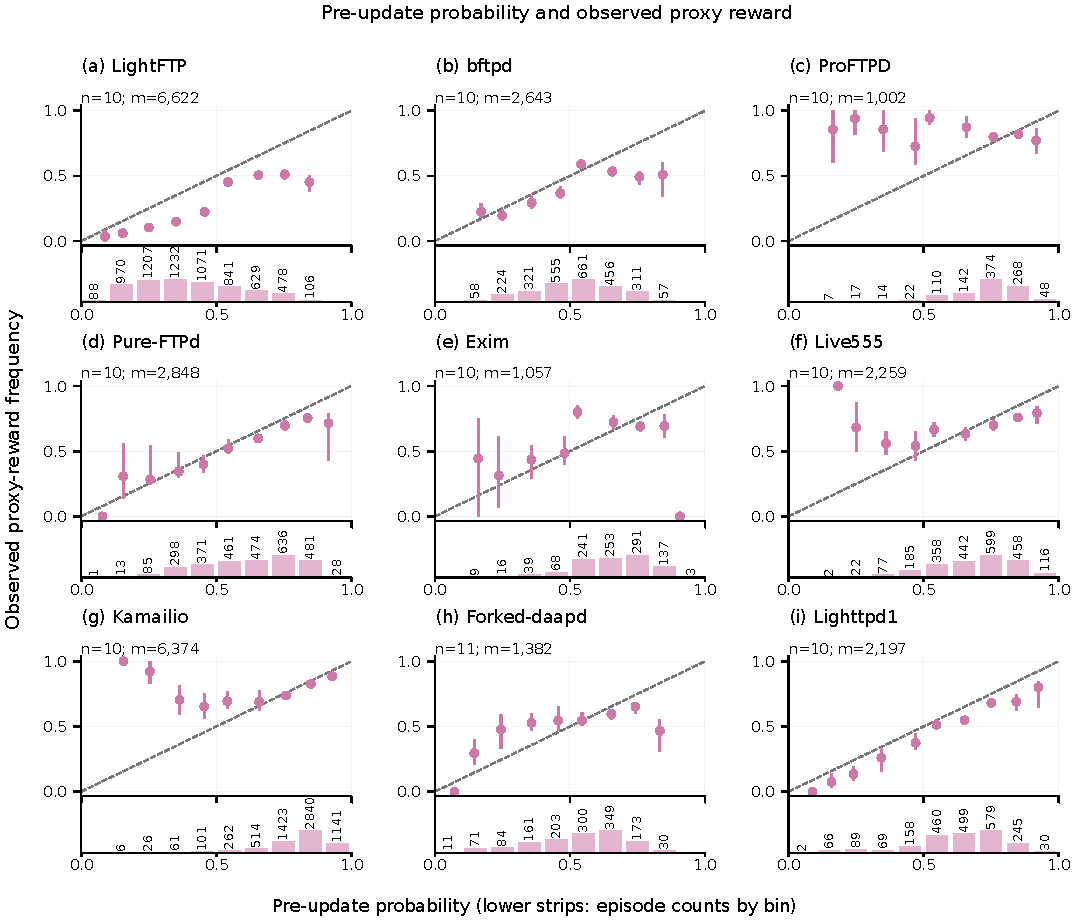
\includegraphics[width=0.90\textwidth]{logged_reward_reliability.pdf}
\caption{E-arm proxy-reward reliability (bin means; 95\% CIs).}
\label{fig:reliability}
\end{figure*}

\subsection{RQ2: Admission records and evidence limits}
The D condition contains 2,227 candidate observations and 2,226 validation trials, with 2,203 reported rejections, 23 durable admissions, and no provisional admissions. One candidate has no corresponding trial; every trial has a corresponding candidate. C and E contain 1,326/1,326 and 746/745 candidates/trials, respectively. C has 1,326 reported durable admissions; E has 736 rejections and 9 durable admissions. These reported decisions do not independently verify queue membership or establish the required 99.9\% observation completeness.

Candidate and admission observations are available for C, D, and E, with target-specific gaps. ProFTPD lacks these observations in D and E despite nonzero model usage. No provisional-lifecycle or repair-outcome observations are available across the 642 records. Reported provisional counts for admission, conversion, and expiration are zero throughout; the rates in \namedref{Table}{tab:mechanisms} therefore describe recorded counters, not verified queue behavior. \namedref{Table}{tab:observed_log_counts} gives D-condition counts, and \namedref{Table}{tab:archive_arms} gives endpoint results. Missing observations establish neither zero conversion rates nor absence of provisional validation or repair.

Recorded dispositions do not independently verify durable queue membership. Without validated candidate-to-descendant links and a paired C--D comparison, promotion latency, downstream productivity, nonproductive retention, and admission false negatives cannot be estimated. Unreconciled usage also prevents attributing code gain to individual candidates or token expenditure. Accordingly, no reduction in queue pollution or improvement in downstream productivity or cost efficiency is claimed. \namedref{Table}{tab:mechanisms} and \namedref{Figure}{fig:dispositions} report observed decisions and latency descriptively; first-failure flags do not independently explain queue retention.

\subsection{RQ3: Exploratory scheduling diagnostics}
C, D, and E contain 56,164, 77,593, and 32,946 state-selection episodes, respectively. Mutation counts range from zero to 18,816 per episode, precluding an equal-energy interpretation of the full samples. Some coverage observations represent distinct instrumentation locations or coverage-based retention events rather than independent source-level code branches. They therefore cannot be combined with terminal code-branch counts or interpreted as the primary reward in Equation~\ref{eq:reward}.

An exploratory equal-energy subset holds the recorded mutation count constant for the corresponding diagnostics in \namedref{Table}{tab:mechanisms}; it does not establish matched target composition, run conditions, or a causal scheduling contrast. Restricting to episodes with exactly 265 mutations, the most frequent nonzero energy value shared by all three arms, leaves 3,986, 6,604, and 1,474 episodes for C, D, and E. Within this subset, mean recorded code edges per episode are 0.009, 0.003, and 0.016, and proxy-reward base rates are 0.004, 0.001, and 0.005: outcomes steeply rise with energy across all arms (episodes above 5,000 mutations are almost always rewarded), so this fixed low energy selects a heavily imbalanced slice. Pre-update predictions are overconfident in this subset (BS 0.240, 0.192, 0.315; ten-bin ECE 0.428, 0.373, 0.516). The posteriors were updated under mixed energies; AP exceeds the recorded base rate (AP 0.012, 0.005, and 0.038 versus base rates near 0.005). These subset diagnostics are exploratory: they condition the logged proxy reward on one energy rather than measuring energy-conditioned calibration, are pooled across targets without clustered uncertainty, and do not replace the per-target full-sample diagnostics in \namedref{Table}{tab:logged_calibration}.

The evaluation includes the calibrated condition E and two discount-factor sensitivity conditions. Heterogeneous observation periods and uncertain effective scheduling policies prevent a matched causal interpretation of E--D. \namedref{Table}{tab:mainresults} reports the recoverable endpoints and AUCs; all 45 main target--arm combinations are represented, including ten E/bftpd observations. End-of-run configuration records verify $\gamma=0.99$ in 66 of the 81 $\gamma=0.99$ observations and $\gamma=1.0$ in 79 of the 91 $\gamma=1.0$ observations; the remaining records carry the fixed-policy configuration at $\gamma=0.995$. Four $\gamma=0.99$ target groups remain below the nominal ten runs (Lighttpd1 6, Live555 7, Kamailio 9, Forked-daapd 9). A calibration benefit requires a prespecified analysis under matched observation periods.

\figref{fig:trajectories} shows code-branch medians and interquartile ranges on a five-minute grid over 0--24 hours from fuzzer startup; the bands are not CIs. Linear interpolation stays within recorded observations, and labels give the contributing $n$ at 24 hours. \namedref{Table}{tab:mainresults} instead integrates each full observed trajectory in branch-hours; cells show branches with actual $n$ above AUC, both as mean $\pm$ SD. Each run contributes only between its first and last observation; time-dependent denominators accompany the figure data. Changes in the set of contributing runs can change an aggregate curve even when individual histories do not decrease. In 127 of the 470 observed trajectories, at least one recorded branch count decreases. The figure preserves these observations without applying a cumulative maximum or otherwise correcting the replay output; both within-run decreases and changing support can produce aggregate decreases.

\figref{fig:posterior_cases} presents three reproducibly selected state histories. For each motivating target, the E run is selected by the lower median terminal branch count, with a deterministic record ordering resolving ties; its two states with the most positive-mutation episodes are shown. Selection uses neither calibration accuracy nor effect direction. Complete histories, including zero-mutation episodes, show pre-update probabilities above the final-selection/frontier-score ratio. Time denotes episode end; lines guide the eye, and colors identify states within each target. Undefined zero-frontier ratios are omitted. These cases illustrate observed behavior without establishing a causal state/code mismatch.



\begin{table*}[!tbp]
\centering\small
\caption{Branch endpoints (top) and AUCs (bottom), mean $\pm$ SD.}
\label{tab:mainresults}
\begin{tabularx}{\textwidth}{l *{5}{>{\centering\arraybackslash}X}}
\toprule
Target & A & B & C & D & E \\
\midrule
LightFTP & \shortstack{71.0$\pm$0.0\,(n=13)\\1758.5$\pm$33.8} & \shortstack{71.3$\pm$0.9\,(n=11)\\1728.1$\pm$36.5} & \shortstack{80.6$\pm$15.5\,(n=10)\\1987.7$\pm$394.1} & \shortstack{71.7$\pm$2.3\,(n=15)\\1780.7$\pm$45.2} & \shortstack{73.9$\pm$4.5\,(n=10)\\1825.0$\pm$107.6} \\
\addlinespace[3pt]
bftpd & \shortstack{486.0$\pm$8.8\,(n=10)\\11868.7$\pm$165.6} & \shortstack{492.2$\pm$14.1\,(n=10)\\12068.6$\pm$323.8} & \shortstack{498.9$\pm$12.2\,(n=10)\\12082.0$\pm$451.0} & \shortstack{502.7$\pm$7.5\,(n=10)\\12267.7$\pm$387.9} & \shortstack{503.7$\pm$7.1\,(n=10)\\12416.6$\pm$220.9} \\
\addlinespace[3pt]
ProFTPD & \shortstack{5053.8$\pm$97.4\,(n=10)\\122652.5$\pm$1730.1} & \shortstack{5205.9$\pm$166.7\,(n=10)\\125217.7$\pm$2989.1} & \shortstack{5446.3$\pm$194.7\,(n=10)\\130538.5$\pm$4511.6} & \shortstack{5428.1$\pm$104.0\,(n=12)\\132539.2$\pm$2868.9} & \shortstack{5469.8$\pm$215.7\,(n=10)\\130564.7$\pm$4604.1} \\
\addlinespace[3pt]
Pure-FTPd & \shortstack{1076.4$\pm$89.6\,(n=11)\\23054.1$\pm$2084.4} & \shortstack{1109.3$\pm$40.0\,(n=10)\\24976.6$\pm$1126.8} & \shortstack{1221.2$\pm$48.9\,(n=10)\\28860.8$\pm$1645.7} & \shortstack{1223.3$\pm$29.7\,(n=10)\\27863.9$\pm$1496.9} & \shortstack{1215.4$\pm$63.7\,(n=10)\\27894.3$\pm$1737.6} \\
\addlinespace[3pt]
Exim & \shortstack{3798.8$\pm$43.3\,(n=10)\\91083.0$\pm$1031.5} & \shortstack{3761.7$\pm$60.4\,(n=10)\\91301.7$\pm$1501.4} & \shortstack{3896.1$\pm$25.6\,(n=10)\\94880.1$\pm$928.3} & \shortstack{3914.9$\pm$20.9\,(n=10)\\93659.0$\pm$573.1} & \shortstack{3858.3$\pm$32.8\,(n=10)\\93123.6$\pm$924.6} \\
\addlinespace[3pt]
Live555 & \shortstack{2893.6$\pm$14.5\,(n=10)\\71127.4$\pm$517.3} & \shortstack{2882.4$\pm$22.0\,(n=10)\\71224.8$\pm$422.5} & \shortstack{3075.7$\pm$34.4\,(n=10)\\73511.0$\pm$562.9} & \shortstack{3067.1$\pm$29.5\,(n=12)\\75436.1$\pm$712.2} & \shortstack{3054.2$\pm$20.5\,(n=10)\\72378.5$\pm$1049.8} \\
\addlinespace[3pt]
Kamailio & \shortstack{10002.6$\pm$144.2\,(n=10)\\242853.7$\pm$2772.6} & \shortstack{10644.3$\pm$96.5\,(n=10)\\257606.8$\pm$2082.0} & \shortstack{10800.6$\pm$129.0\,(n=10)\\260260.9$\pm$2942.4} & \shortstack{10631.2$\pm$472.9\,(n=12)\\254332.1$\pm$9492.1} & \shortstack{10830.0$\pm$91.3\,(n=10)\\259377.2$\pm$2649.6} \\
\addlinespace[3pt]
Forked-daapd & \shortstack{2330.8$\pm$60.0\,(n=10)\\54453.2$\pm$1494.1} & \shortstack{2169.6$\pm$113.0\,(n=10)\\49393.2$\pm$3335.9} & \shortstack{2585.4$\pm$86.2\,(n=10)\\61776.8$\pm$1863.7} & \shortstack{2670.2$\pm$87.3\,(n=12)\\63646.7$\pm$1977.0} & \shortstack{2609.0$\pm$96.6\,(n=11)\\61843.9$\pm$1570.4} \\
\addlinespace[3pt]
Lighttpd1 & \shortstack{1940.7$\pm$21.2\,(n=10)\\46909.4$\pm$235.7} & \shortstack{1884.1$\pm$25.3\,(n=10)\\45075.8$\pm$729.3} & \shortstack{2145.0$\pm$69.8\,(n=10)\\53003.8$\pm$1613.7} & \shortstack{2126.7$\pm$15.7\,(n=11)\\51223.2$\pm$621.1} & \shortstack{2068.1$\pm$44.5\,(n=10)\\50385.1$\pm$941.3} \\
\bottomrule
\end{tabularx}
\end{table*}

\begin{figure*}[!tbp]
\centering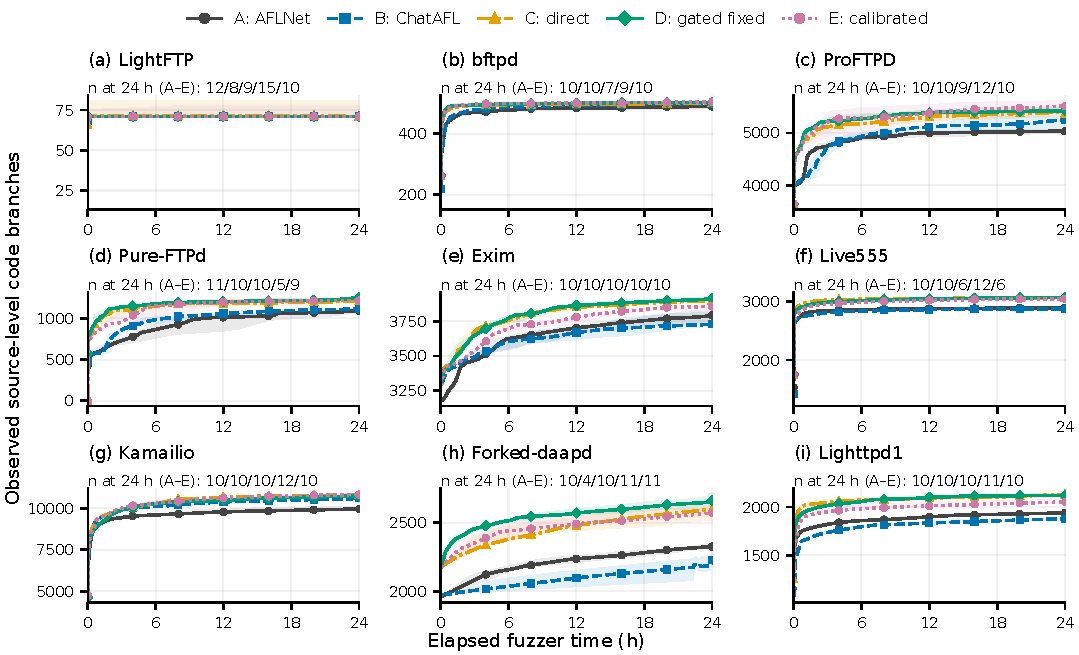
\includegraphics[width=\textwidth]{coverage_trajectories.pdf}
\caption{A--E code-branch trajectories (median and interquartile range).}
\label{fig:trajectories}
\end{figure*}

\begin{figure*}[!tbp]
\centering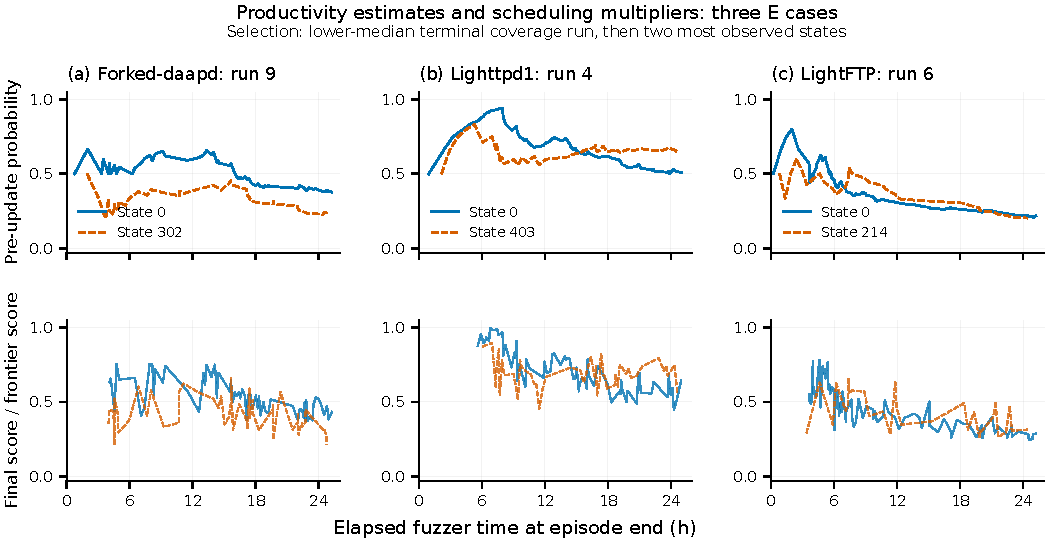
\includegraphics[width=\textwidth]{posterior_cases.pdf}
\caption{E-arm pre-update probabilities (top) and scheduling multipliers (bottom).}
\label{fig:posterior_cases}
\end{figure*}

\begin{table*}[!tbp]
\centering\footnotesize
\caption{C/D/E admission records and exploratory reward diagnostics.}
\label{tab:mechanisms}
\begin{tabularx}{\textwidth}{>{\raggedright\arraybackslash}p{0.19\textwidth} *{3}{>{\centering\arraybackslash}p{0.14\textwidth}} Y}
\toprule
Metric & C & D & E & Denominator / interpretation \\
\midrule
Candidate records & 1,326 & 2,227 & 746 & Within-run distinct candidates. \\
Trial records & 1,326 & 2,226 & 745 & Within-run distinct trials. \\
Reject / durable labels & 0 / 1,326 & 2,203 / 23 & 736 / 9 & Reported trial outcomes. \\
First failed $P/U/R$ & 0 / 1,208 / 0 & 0 / 2,071 / 0 & 0 / 698 / 0 & Trial denominator; first false $P$, $U$, or $R$. \\
Direct durable rate & 100.0\% (1,326/1,326) & 1.0\% (23/2,227) & 1.2\% (9/746) & Durable labels / generated candidates. \\
State-only provisional rate & disabled & 0.0\% (0/2{,}227) & 0.0\% (0/746) & All candidates; disabled for C. \\
Provisional conversion / expiration & disabled & none (0 admitted) & none (0 admitted) & Provisional admissions; retain pending/censored cases. \\
Trial latency (ms) & 439.2$\pm$405.9 ($n=67$) & 403.6$\pm$574.6 ($n=81$) & 806.5$\pm$554.0 ($n=62$) & Within-run trial means; contributing runs only. \\
Recorded code-edge gain / episode & 0.009 ($n=3{,}986$) & 0.003 ($n=6{,}604$) & 0.016 ($n=1{,}474$) & 265-mutation subset; recorded coverage gain. \\
BS / ECE / AP & 0.240 / 0.428 / 0.012 & 0.192 / 0.373 / 0.005 & 0.315 / 0.516 / 0.038 & 265-mutation subset; pooled proxy reward; see \namedref{Table}{tab:logged_calibration}. \\
\bottomrule
\end{tabularx}
\end{table*}

\begin{figure*}[!tbp]
\centering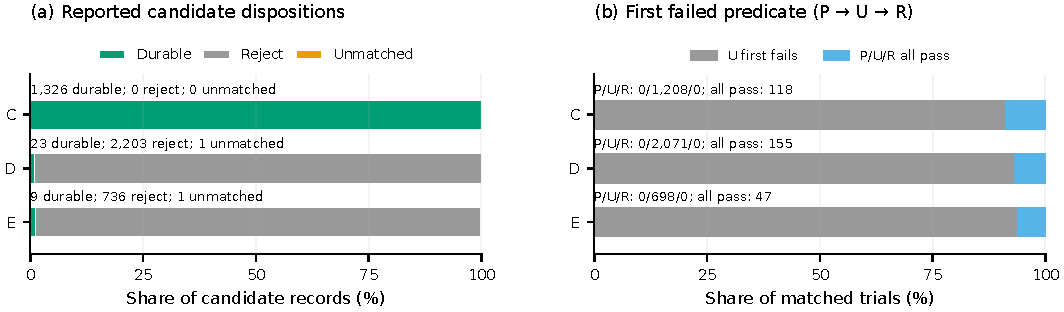
\includegraphics[width=\textwidth]{candidate_dispositions.pdf}
\caption{C/D/E reported dispositions (left) and first $P/U/R$ failures (right).}
\label{fig:dispositions}
\end{figure*}

\subsection{RQ5: Recorded costs and interpretation limits}
\namedref{Table}{tab:observed_costs} reports model calls and token usage for D by target; supporting results also give C/E ranges and means. Model calls range from 52 to 248 per D run, so the stated limit of 64 does not establish a campaign-wide ceiling. Usage estimates have not been independently reconciled with provider charges and may omit the final observation interval.

The recorded end-of-run configurations identify a model name, grammar/plateau temperatures of 0.5/1.2, top-$p$ of 1.0, an output limit of 4096 tokens, a call cap of 64, and a token-limit setting of 0; these values appear in every C/D/E and $\gamma$-sensitivity archive and are consolidated in \namedref{Table}{tab:llm}. A model name does not uniquely identify the inference version, and ChatAFL-arm archives embed no equivalent record. Uncertainty in effective conditions and resource measurement limits interpretation; these values do not establish the shared confirmatory settings required of B--E.

Candidate token fields do not necessarily cover all call classes or retries; summing them is not total campaign cost. Low-activation targets, high-rejection targets, token outliers, saturation, and regressions must remain in the final analysis. Low activation may reflect productive mutation or a restrictive trigger; high rejection may reflect either useful gating or false negatives. Both need mechanism evidence.

% Generated from current selected benchmark LoopFuzz D archives.
\begin{table}[!tbp]
\centering\small
\caption{D-arm cost ranges; total tokens = input + output (k = 1,000).}
\label{tab:observed_costs}
\begin{tabular}{lrr}
\toprule
Target & Model calls & Total tokens (k) \\
\midrule
LightFTP & 59--161 & 106.0--224.7 \\
bftpd & 199--248 & 198.0--301.8 \\
ProFTPD & 188--192 & 170.1--198.8 \\
Pure-FTPd & 207--242 & 200.2--264.1 \\
Exim & 106--123 & 109.4--151.0 \\
Live555 & 123--189 & 264.1--433.1 \\
Kamailio & 56--108 & 157.0--285.5 \\
Forked-daapd & 52--163 & 103.4--540.9 \\
Lighttpd1 & 131--187 & 168.5--252.5 \\
\bottomrule
\end{tabular}
\end{table}


\namedref{Figures}{fig:cost} and~\ref{fig:callcost} plot reported token usage and model calls against terminal code branches for 376 B--E runs, using target-specific scales. Tokens combine prompt and completion counts and are displayed in thousands (k). Comparable AFLNet usage measurements are unavailable; calls measure neither token expenditure nor CPU time. These views reveal dispersion and usage ranges without estimating a causal return per token or call. Measured CPU-hours and controlled A--E CVE recall remain unavailable. The case-level replays in Section~\ref{sec:cve} do not supply those cost--performance axes.



\begin{figure*}[!tbp]
\centering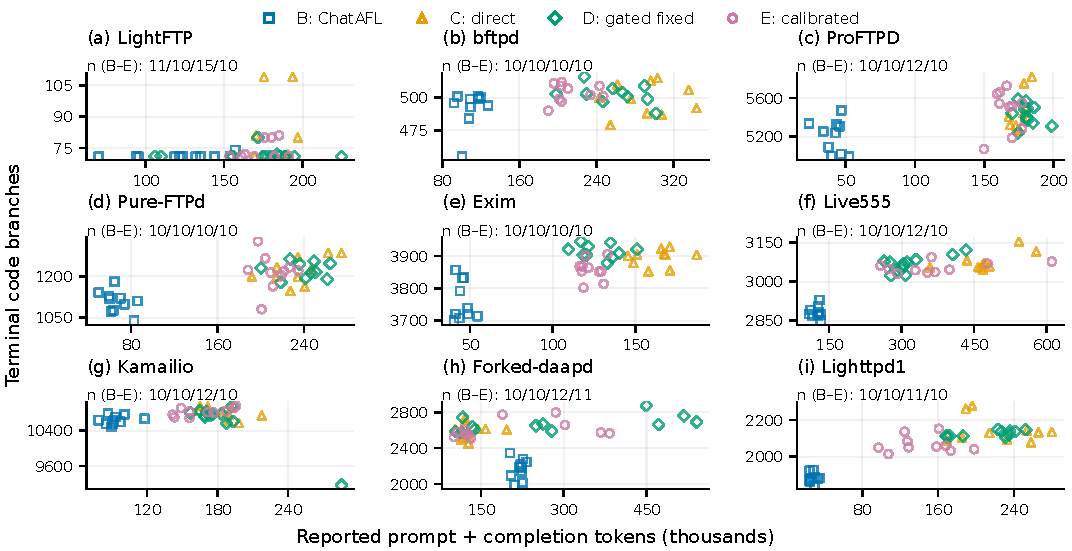
\includegraphics[width=\textwidth]{token_cost_coverage.pdf}
\caption{Code-branch endpoints versus reported tokens, by target and arm.}
\label{fig:cost}
\end{figure*}

\begin{figure*}[!tbp]
\centering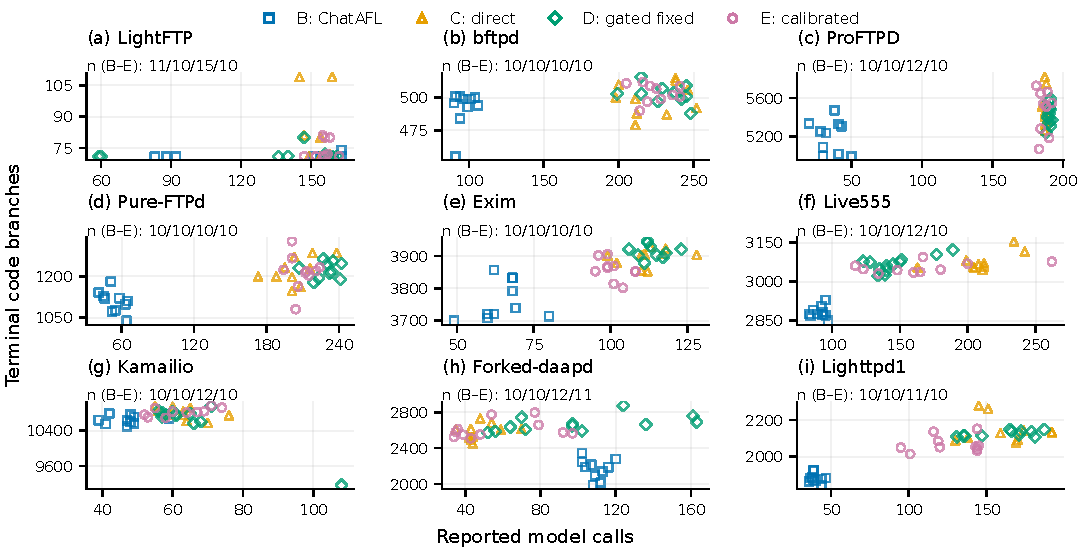
\includegraphics[width=\textwidth]{call_cost_coverage.pdf}
\caption{Code-branch endpoints versus reported calls, by target and arm.}
\label{fig:callcost}
\end{figure*}



Repair remains an optional, unquantified feature. No repair outcomes were recorded, and the study reports no repair ablation, effectiveness estimate, or repair-specific cost comparison.

\section{Vulnerability Replay Evidence and Rediscovery Protocol}
\label{sec:cve}
The vulnerability study comprises four cases: three associated with CVE identifiers and one SMARTPL availability failure without a CVE. Each case has a report and a triggering input; three have direct execution evidence, and ProFTPD also has a reported patched-version comparison. \namedref{Tables}{tab:cve} and~\ref{tab:cveresults} summarize these observations. Case identities, versions, and replay counts follow the original reports; incomplete patch and experimental-configuration evidence prevents independent verification of every version pair.

\subsection{Case identity and evidence provenance}
We distinguish a direct execution observation (L) from a replay result stated only in a case report (R). A report can contain additional trials not represented by the available execution evidence. Duplicate diagnostic observations do not constitute independent trials. Input identity and byte length are retained in the supporting evidence. This retrospective analysis involves no additional target executions. \namedref{Table}{tab:cve} identifies the reported versions, triggering conditions, and comparative evidence.

\begin{table*}[!tbp]
\centering\small
\caption{Vulnerability cases and supporting evidence (L: direct observation; R: report).}
\label{tab:cve}
\begin{tabularx}{\textwidth}{@{}>{\raggedright\arraybackslash}p{0.20\textwidth} >{\raggedright\arraybackslash}p{0.19\textwidth} Y Y@{}}
\toprule
Case / interface & Reported vulnerable version & Trigger evidence / oracle & Patch or control evidence \\
\midrule
\mbox{CVE-2023-51713}\newline ProFTPD / FTP & Reported vulnerable build; 65,535-byte buffer. & 60,006-byte input; ASan heap-buffer-overflow (L). & Security patch: three rejections, no ASan (L). \\
\addlinespace[3pt]
\mbox{CVE-2026-38998}\newline LIVE555 / RTSP & Campaign: 2023.05.10; report: 2026.02.26 (R). & 728-byte public PoC; use-after-free (L). & Local patch: 1/1 triggers (R); upstream comparison unavailable. \\
\addlinespace[3pt]
\mbox{CVE-2026-39863}\newline Kamailio / SIP over TCP & Reported vulnerable build; TCP required. & 278-byte input; parsed Content-Length $-10$ (L). & Patched: 0/253 negative-value outcomes; guard observed (L). \\
\addlinespace[3pt]
SMARTPL availability case\newline forked-daapd / HTTP & Reported version 27.2. & 148-byte input; unresponsive service, live process (R). & No patched replay/CVE; removal reported in 28.4. \\
\bottomrule
\end{tabularx}
\end{table*}

For ProFTPD, the reported defect is an out-of-bounds read during FTP command processing, supported by an ASan heap-buffer-overflow observation. The 60,006-byte reproducer caused a one-byte read beyond a 65,568-byte region. The oracle uses a 65,535-byte command buffer; the report states that the default 512-byte configuration does not expose the same error to ASan. The result is therefore conditional on this setting. The full replay in \namedref{Table}{tab:cveresults} uses a purpose-built version pair at the campaign's base commit whose only difference is the minimal upstream fix; on that pair, 172 of 233 campaign crash inputs trigger the \texttt{make\_ftp\_cmd} predicate on the vulnerable side and none of 242 activate ASan on the patched side. This supplies differential replay evidence with verified version identity for the pair, while the earlier three-trial fix batch remains separate. Earlier reported replays yielded 1/1 seed, 1/1 fuzzer-crash, and 3/3 batch-crash reproductions; the separate fix batch yielded 0/3 using the same input and buffer.

For LIVE555, direct diagnostic evidence supports a use-after-free triggered by the public PoC. A duplicated observation is treated as one diagnostic signature rather than independent replication. The report attributes fuzzer-generated inputs to the same memory-lifetime failure. It gives 1/1 public-PoC reproduction, 3/3 repeats for each of three fuzzer inputs, a later 8/9 aggregate, and 1/1 persistence after a local patch. The fuzzer-generated reproducer, complete memory-lifetime evidence, and individual trial outcomes are unavailable. The public PoC supports replay validation, but does not demonstrate independent rediscovery by the evaluated controller or independently establish cross-version CVE attribution.

For Kamailio, a negative parsed Content-Length supports the reported integer-overflow condition. The trigger requires TCP and is not assessed by the UDP-only benchmark condition. The full census in \namedref{Table}{tab:cveresults} replays every queue entry carrying an oversized Content-Length on a purpose-built pair at the campaign's base commit whose only difference is the upstream guard: 102 of 253 entries produce the negative-value artifact on the vulnerable side, none do on the patched side, and the patched build logs the upstream guard for 193 of 253. Earlier reported batches remain separate: 1/1 seed and 3/4, 19/20, 19/20, and 50/51 selected inputs. The prior local-guard observation is also separate. Queue entries are fuzzer-generated artifacts, so the census measures predicate yield over retained inputs, not rediscovery. An earlier unsupported 20/20 versus 0/20 claim is excluded from quantitative results. 

For SMARTPL, the 148-byte input reportedly causes lexer errors and a failed health probe while the process remains alive. Reported repeats comprise 5/5 advisory trials, 3/3 trials with a 48-message seed, and a later 1/1 replay. None of the five recorded campaign hangs reproduces this condition; a CVE and verified patched counterpart remain unavailable. Parser removal in version 28.4 is reported, not a verified patched replay.

\subsection{Replay outcomes and their denominators}
\namedref{Table}{tab:cveresults} summarizes the replay outcomes; earlier reported batches remain separate in the case descriptions. A numerator counts replay attempts or selected queue inputs satisfying that case's predicate; the denominator is the number tested. These are not independent 12-hour fuzzer runs, and the main experiment's nominal $N=10$ is not substituted for the actual replay denominator. Selected batches, per-input repeats, and later aggregate counts may overlap; they are not pooled into one success rate. In particular, 19/20 selected inputs is not 95\% campaign recall, and 8/9 LIVE555 replays is below the prospective 95\% stability threshold.

Three complete-input replays extend these batches (September 30 observations). First, every crash input recorded by the two 24-hour ProFTPD LoopFuzz campaigns (233 in-campaign inputs: 121 and 112 per run; 9 teardown inputs) was replayed once against the vulnerable and patched images of the verified \texttt{o-pftp-01} pair (same base commit, minimal upstream fix). On the vulnerable image, 172 of the 233 in-campaign inputs trigger the ASan heap-buffer-overflow predicate in \texttt{make\_ftp\_cmd}; all 172 carry that frame and no other signature appears. The patched image shows no ASan activation for any of the 242 inputs. The 61 non-reproducing inputs and the 9 teardown inputs may require campaign state that a standalone replay does not reconstruct; the in-campaign forensic sidecars recorded almost no usable ASan output, so the pair replay is the authoritative verdict. Second, all 88 LIVE555 campaign crash inputs were replayed against the campaign build, which contains no sanitizer: 82 terminate the server and 6 do not. This establishes reproduction on that build only; without a patched counterpart or sanitizer output it does not attribute the crashes to the use-after-free. Third, all 253 Kamailio queue entries with Content-Length $\geq 2^{31}$ were replayed on the \texttt{o-kam-01} pair: 102 produce the negative-value artifact on the vulnerable build and none on the patched build. The two runs contributed 77 and 176 entries, with yields of 36/77 and 66/176. Overflow values include $-2147483648$, $-1$, and $-954437177$; 151/253 entries do not produce the artifact, with ordering and parse-path explanations unresolved. All three replays are artifact-level measurements: they provide no arm-level recall, time-to-trigger, or cost denominators.

\begin{table*}[!tbp]
\centering\small
\caption{Replay outcomes and controls; original denominators retained.}
\label{tab:cveresults}
\begin{tabularx}{\textwidth}{@{}>{\raggedright\arraybackslash}p{0.20\textwidth} Y Y Y@{}}
\toprule
Case & Replay outcome & Control outcome & Evidence limit \\
\midrule
\mbox{CVE-2023-51713} & 172/233 ASan triggers (L). & Patched: 0/242 ASan activations (L). & Artifact replay; campaign recall unmeasured. \\
\addlinespace[3pt]
\mbox{CVE-2026-38998} & 82/88 server terminations (L). & Local patch: 1/1 triggers (R). & No sanitizer or verified patched build. \\
\addlinespace[3pt]
\mbox{CVE-2026-39863} & 102/253 negative-value outcomes (L). & Patched: 0/253; guard: 193/253 (L). & Selected queue entries; campaign recall unmeasured. \\
\addlinespace[3pt]
SMARTPL availability case & Advisory: 5/5; seed: 3/3; later: 1/1 (R). & Campaign hangs: 0/5 matching outcomes (R). & Known-input replay; no patch or CVE. \\
\bottomrule
\end{tabularx}
\end{table*}

Additional reported crashes and campaigns cannot be linked to the primary benchmark and ablation observations. Crash totals do not count unique vulnerabilities, and durations such as 60 or 1,540 minutes do not specify time to first trigger. Associations among reproducing inputs, verified A--E conditions, model information exposure, and independent root causes are incomplete. The replay outcomes therefore do not establish arm-specific discovery probabilities, novel CVEs, or admission/calibration gains.

\subsection{Controlled rediscovery still to be measured}
Confirmatory rediscovery requires a vulnerable version and the same version with a minimal security patch, holding dependencies, instrumentation, settings, and input compatibility constant. Each case needs a network-reachable trigger, independent reached/triggered criteria, reproducible initial conditions, and a validated patch comparison. The proposed six-case pilot across at least three protocols, followed by expansion toward twelve, remains incomplete. Eligibility requires at least 95\% observed oracle repeatability in a declared validation set, no activation after patching, reproducible experimental preparation, and information separation. The four cases do not constitute six qualified version pairs; a small all-success replay batch does not establish an underlying success probability of at least 95\%.

Information-controlled campaigns must exclude CVE identifiers, advisories, public PoCs, and patch contents from model inputs and campaign seeds, while retaining anonymous oracle IDs in separate benchmark metadata. The public PoC and known triggers in this collection are validation inputs; their replay is not evidence of information-controlled rediscovery. Source-level trigger conditions, sanitizer reports with patch validation, and protocol invariants distinguish reaching relevant code from actually triggering a defect. Experiments require isolated target networks and reset between trials; these are protocol requirements, not properties inferred from the reports.

For each CVE and arm, the formal plan retains ten independent runs and a 12-hour deadline, prespecified before execution. Deadline recall, time-to-trigger, reached-but-not-triggered counts, patched-target activation, executions/coverage/tokens before trigger, and recall per CPU-hour or 100,000 tokens remain unavailable for the controlled A--E comparison. Nontriggers require right-censoring records, and interrupted runs require separate failure accounting. The available replay batches do not define those risk sets, so Kaplan--Meier estimates or arm-level security-effectiveness claims are not reported.

\section{Discussion}
\subsection{What calibration can and cannot repair}
The controller calibrates the instrumental utility of an observed state proxy; it does not recover or verify semantic protocol state. If one response identifier aliases several server states, a single productivity estimate averages them. Reweighting the identifier cannot reconstruct lost distinctions. Richer parsing or internal-state instrumentation addresses different aspects at the cost of adapter complexity and deployment effort.

Low productivity can arise from a poor response proxy, saturated coverage, restrictive grammar, inadequate seeds, or insufficient energy. Independent reward prevents IPSM novelty from certifying itself but does not automatically diagnose these causes. The boundary analysis includes aliasing, cold start, phase, and target-specific regressions.

A fixed provisional horizon can discard a bridge whose payoff requires more descendants. Shadow validation and horizon sensitivity would help quantify this risk, but neither is available here; expired or rejected candidates are not assumed worthless. Likewise, $U/R$ may exclude useful error-handling inputs. Independent oracle retention is a design requirement, while its experimental adequacy and admission false negatives remain unverified.

\subsection{Cost, nonstationarity, and provider variability}
Selection-indexed discounting can retain stale evidence for rarely selected states. Priors and the exploration floor preserve opportunities without guaranteeing fast identification. When code coverage saturates, nearly every reward may be zero, and calibration may offer little benefit.

Model-service nondeterminism persists despite identical prompts and nominal parameters. A shared model name may correspond to different inference versions, repeated requests affect costs, and target responses alter later prompts. Equal-policy/equal-cap comparisons control declared resources; actual usage and cost-matched analysis characterize the remaining tradeoffs. Replay assesses decisions under fixed conditions rather than reproducing an adaptive campaign.

\begin{table*}[!tbp]
\centering\small
\caption{Validity threats, required controls, and evidence limits.}
\label{tab:threats}
\begin{tabularx}{\textwidth}{l Y Y}
\toprule
Dimension & Required control & Current limitation \\
\midrule
Internal & Admission-only C--D; scheduling-only E--D; repair off; matched initial states. & Missing observations; uncertain decision order. \\
Construct & Separate code branches, IPSM state edges, bitmap counts, and oracle outcomes. & Proxies incompletely measure intended criteria. \\
Statistical & Repeated runs; test families; effect sizes; clustered/hierarchical CIs; censoring. & Unequal durations; no confirmatory effects. \\
Selection & Intention-to-run accounting; prespecified infrastructure repetitions. & Unobserved planned runs; independence uncertain. \\
Reproducibility & Match versions, settings, seeds, prompts, and measurements. & Unresolved model versions; incomplete provenance. \\
External & Multiple targets/protocols; boundary cases; adapter assumptions. & Encrypted/opaque binary protocols untested. \\
Security & Minimal patch pairs; independent triggers; information isolation. & Controlled A--E/patch-pair evidence incomplete; pretraining leakage unresolved. \\
\bottomrule
\end{tabularx}
\end{table*}

\subsection{Evidence required for confirmatory claims}
A confirmatory calibration claim requires nondegenerate predictions, reduced investment in branch-unproductive Forked-daapd states when present, and no systematic suppression of Lighttpd1 solely because of limited IPSM novelty. It also requires acceptable throughput on at least three pilot targets and better predictive diagnostics than the shared prequential base-rate reference. D-condition productivity estimates provide an additional diagnostic; the uncalibrated queue-yield ratio is not a probability. An E--D difference must be supported by a plausible measured mechanism. These are prospective eligibility criteria rather than completed significance tests.

In this study, calibration is exploratory, repair is unquantified, and the empirical scope is an integrated-system boundary analysis. Missing validation is not a measured null effect. A later admission or calibration claim requires independent supporting evidence; a rediscovery claim requires controlled campaigns rather than replay alone. Parameters and analysis decisions must be fixed before confirmatory observation.

The planned confirmatory evidence comprises D--C and E--D estimates, complete candidate-level measurements, at least nine targets, twenty runs per core arm, and a reproducible historical benchmark of approximately eight to twelve vulnerabilities. The four replay cases do not meet that benchmark requirement. These are intended sample sizes and coverage criteria, not achieved results.

\section{Threats to Validity}
\namedref{Table}{tab:threats} summarizes the controls and remaining evidence limits.
\label{sec:threats}


The analysis is retrospective. Equivalence between the assessed system and every experimental version is unverified, so methodological concerns and observed outcomes retain separate evidential status. A nonsignificant adjusted comparison does not establish equivalence, and favorable endpoints do not identify a mechanism when duration, resources, or effective procedures differ. Admission, calibration, and rediscovery each require independent supporting evidence.

Benchmark properties can change the relative ranking of fuzzers: initial seed coverage and execution speed are empirically consequential covariates~\cite{benchmarkproperties}. Consequently, a favorable endpoint under unequal experimental conditions cannot isolate the admission or scheduling effect. Mutation-based assessment offers a complementary fault-oriented perspective~\cite{mutationassessment2023}; here, code coverage and IPSM growth are kept separate from independently verified vulnerability outcomes.

\section{Conclusion}
LoopFuzz is presented as an integrated controller design with a retrospective analysis of its evidence boundaries. The proposed admission contract separates code progress from IPSM novelty and gives state-only proposals a bounded provisional budget. Productivity calibration is an exploratory scheduling mechanism; it does not recover semantic protocol states.

The available observations describe coverage, model usage, admission labels, and proxy-reward behavior under incomplete operational validation. Four vulnerability cases add replay evidence with differing patch support. These measurements do not establish reduced queue pollution, improved downstream productivity, greater cost efficiency, or improved rediscovery. The contribution is the controller specification and a documented assessment of the evidence needed to validate its intended benefits; no quantitative repair effect is claimed.

\section*{CRediT authorship contribution statement}
Author contribution roles remain to be confirmed by all authors before submission.
\section*{Declaration of competing interest}
The competing-interest declaration remains to be confirmed by all authors.
\section*{Funding}
Funding information remains to be confirmed by all authors.
\section*{Data availability}
The 642 experimental records and four vulnerability case studies are accompanied by trial-level measurements, version and input provenance, and numerical figure data. Public access and persistent identifiers remain unspecified; exact reproduction of model-service responses is not claimed.
\section*{Declaration of generative AI and AI-assisted technologies in the manuscript preparation process}
OpenAI Codex assisted language revision, organization, figure preparation, and consistency assessment. The authors remain responsible for scientific accuracy and the final disclosure.

\appendix
\setcounter{table}{0}
\renewcommand{\theHtable}{appendix.\Alph{section}.\arabic{table}}
\section{Complete descriptive results}
\label{sec:archive_appendix}
\namedref{Table}{tab:archive_arms} reports all observations underlying the descriptive comparisons, using the same values and sample SDs as the main results. Sample sizes are shown once per row; unavailable target--arm conditions are not imputed.
% Generated from current Key_Experiment archives on 2026-09-30.
\begingroup
\small
\setlength{\tabcolsep}{1.6pt}
\renewcommand{\arraystretch}{1.0}
\noindent Row IDs = arm + target number. Arms A--E follow the main text; $E_{99}$: $\gamma=0.99$; $E_{100}$: $\gamma=1.0$.
\par\smallskip
\noindent\begin{tabularx}{\columnwidth}{@{}YYY@{}}
1: LightFTP & 4: Pure-FTPd & 7: Kamailio \\
2: bftpd & 5: Exim & 8: Forked-daapd \\
3: ProFTPD & 6: Live555 & 9: Lighttpd1 \\
\end{tabularx}
\par\smallskip
\noindent AUC: branch-hours; IPSM: state edges. Status: C, completed; X, exit 137 near limit; S, SIGABRT; O, reported OOM. Labels do not verify causes. Missing combinations are unobserved, not zero.
\par\smallskip
\captionof{table}{Target--arm coverage (mean $\pm$ SD; actual $n$, nominal $N=10$).}
\label{tab:archive_arms}
\tablefirsthead{\toprule ID & $n$ & Branches & AUC & IPSM & Status \\ \midrule}
\tablehead{\multicolumn{6}{l}{Table~\thetable\ (continued)}\\ \toprule ID & $n$ & Branches & AUC & IPSM & Status \\ \midrule}
\tabletail{\bottomrule}
\tablelasttail{\bottomrule}
\noindent\begin{supertabular}{@{}lrrrrl@{}}
A1 & 13 & 71.0$\pm$0.0 & 1758.5$\pm$33.8 & 187.3$\pm$11.3 & C:13 \\
A2 & 10 & 486.0$\pm$8.8 & 11868.7$\pm$165.6 & 163.1$\pm$15.4 & C:10 \\
A3 & 10 & 5053.8$\pm$97.4 & 122652.5$\pm$1730.1 & 190.5$\pm$27.9 & C:10 \\
A4 & 11 & 1076.4$\pm$89.6 & 23054.1$\pm$2084.4 & 236.5$\pm$26.7 & C:11 \\
A5 & 10 & 3798.8$\pm$43.3 & 91083.0$\pm$1031.5 & 88.8$\pm$5.2 & C:10 \\
A6 & 10 & 2893.6$\pm$14.5 & 71127.4$\pm$517.3 & 96.1$\pm$8.6 & C:10 \\
A7 & 10 & 10002.6$\pm$144.2 & 242853.7$\pm$2772.6 & 109.4$\pm$9.7 & C:10 \\
A8 & 10 & 2330.8$\pm$60.0 & 54453.2$\pm$1494.1 & 21.6$\pm$2.1 & C:10 \\
A9 & 10 & 1940.7$\pm$21.2 & 46909.4$\pm$235.7 & 17.7$\pm$2.5 & C:10 \\
B1 & 11 & 71.3$\pm$0.9 & 1728.1$\pm$36.5 & 195.1$\pm$14.6 & C:11 \\
B2 & 10 & 492.2$\pm$14.1 & 12068.6$\pm$323.8 & 167.1$\pm$12.5 & C:10 \\
B3 & 10 & 5205.9$\pm$166.7 & 125217.7$\pm$2989.1 & 150.0$\pm$18.5 & C:10 \\
B4 & 10 & 1109.3$\pm$40.0 & 24976.6$\pm$1126.8 & 186.0$\pm$31.5 & C:10 \\
B5 & 10 & 3761.7$\pm$60.4 & 91301.7$\pm$1501.4 & 115.8$\pm$13.5 & C:10 \\
B6 & 10 & 2882.4$\pm$22.0 & 71224.8$\pm$422.5 & 143.8$\pm$8.8 & C:10 \\
B7 & 10 & 10644.3$\pm$96.5 & 257606.8$\pm$2082.0 & 106.5$\pm$6.8 & C:10 \\
B8 & 10 & 2169.6$\pm$113.0 & 49393.2$\pm$3335.9 & 17.7$\pm$4.9 & C:10 \\
B9 & 10 & 1884.1$\pm$25.3 & 45075.8$\pm$729.3 & 14.3$\pm$3.1 & C:10 \\
C1 & 10 & 80.6$\pm$15.5 & 1987.7$\pm$394.1 & 210.6$\pm$8.3 & C:10 \\
C2 & 10 & 498.9$\pm$12.2 & 12082.0$\pm$451.0 & 217.9$\pm$13.8 & C:6,X:4 \\
C3 & 10 & 5446.3$\pm$194.7 & 130538.5$\pm$4511.6 & 300.7$\pm$29.1 & X:9,C:1 \\
C4 & 10 & 1221.2$\pm$48.9 & 28860.8$\pm$1645.7 & 328.5$\pm$22.5 & C:7,X:3 \\
C5 & 10 & 3896.1$\pm$25.6 & 94880.1$\pm$928.3 & 150.9$\pm$9.5 & C:10 \\
C6 & 10 & 3075.7$\pm$34.4 & 73511.0$\pm$562.9 & 166.8$\pm$9.3 & C:10 \\
C7 & 10 & 10800.6$\pm$129.0 & 260260.9$\pm$2942.4 & 139.2$\pm$9.8 & C:9,X:1 \\
C8 & 10 & 2585.4$\pm$86.2 & 61776.8$\pm$1863.7 & 22.3$\pm$2.2 & C:8,S:2 \\
C9 & 10 & 2145.0$\pm$69.8 & 53003.8$\pm$1613.7 & 32.1$\pm$5.0 & C:10 \\
D1 & 15 & 71.7$\pm$2.3 & 1780.7$\pm$45.2 & 207.0$\pm$17.0 & C:15 \\
D2 & 10 & 502.7$\pm$7.5 & 12267.7$\pm$387.9 & 226.7$\pm$14.0 & C:10 \\
D3 & 12 & 5428.1$\pm$104.0 & 132539.2$\pm$2868.9 & 305.3$\pm$20.3 & C:12 \\
D4 & 10 & 1223.3$\pm$29.7 & 27863.9$\pm$1496.9 & 321.4$\pm$11.1 & C:10 \\
D5 & 10 & 3914.9$\pm$20.9 & 93659.0$\pm$573.1 & 152.7$\pm$9.3 & C:10 \\
D6 & 12 & 3067.1$\pm$29.5 & 75436.1$\pm$712.2 & 170.1$\pm$11.1 & C:12 \\
D7 & 12 & 10631.2$\pm$472.9 & 254332.1$\pm$9492.1 & 128.2$\pm$26.6 & C:12 \\
D8 & 12 & 2670.2$\pm$87.3 & 63646.7$\pm$1977.0 & 22.8$\pm$2.9 & C:12 \\
D9 & 11 & 2126.7$\pm$15.7 & 51223.2$\pm$621.1 & 28.9$\pm$2.7 & C:11 \\
E1 & 10 & 73.9$\pm$4.5 & 1825.0$\pm$107.6 & 210.9$\pm$9.3 & C:10 \\
E2 & 10 & 503.7$\pm$7.1 & 12416.6$\pm$220.9 & 215.8$\pm$7.5 & C:9,O:1 \\
E3 & 10 & 5469.8$\pm$215.7 & 130564.7$\pm$4604.1 & 307.8$\pm$21.3 & X:5,C:5 \\
E4 & 10 & 1215.4$\pm$63.7 & 27894.3$\pm$1737.6 & 311.6$\pm$22.4 & X:5,C:5 \\
E5 & 10 & 3858.3$\pm$32.8 & 93123.6$\pm$924.6 & 138.6$\pm$14.3 & C:10 \\
E6 & 10 & 3054.2$\pm$20.5 & 72378.5$\pm$1049.8 & 162.1$\pm$4.4 & C:10 \\
E7 & 10 & 10830.0$\pm$91.3 & 259377.2$\pm$2649.6 & 130.9$\pm$9.0 & C:10 \\
E8 & 11 & 2609.0$\pm$96.6 & 61843.9$\pm$1570.4 & 21.8$\pm$1.7 & C:11 \\
E9 & 10 & 2068.1$\pm$44.5 & 50385.1$\pm$941.3 & 27.1$\pm$4.4 & C:10 \\
$E_{99}$1 & 10 & 71.9$\pm$2.8 & 1785.4$\pm$78.3 & 210.6$\pm$12.4 & C:10 \\
$E_{99}$2 & 10 & 496.8$\pm$9.2 & 12210.9$\pm$353.6 & 224.0$\pm$9.8 & C:8,X:2 \\
$E_{99}$3 & 10 & 5504.6$\pm$132.2 & 134386.6$\pm$3705.3 & 310.5$\pm$19.2 & C:9,X:1 \\
$E_{99}$4 & 10 & 1219.4$\pm$26.3 & 28302.9$\pm$964.5 & 310.5$\pm$19.8 & C:10 \\
$E_{99}$5 & 10 & 3856.3$\pm$26.9 & 94717.9$\pm$787.4 & 158.9$\pm$13.5 & X:3,C:7 \\
$E_{99}$6 & 7 & 3091.9$\pm$19.9 & 75920.1$\pm$441.3 & 161.3$\pm$6.8 & C:7 \\
$E_{99}$7 & 9 & 10852.9$\pm$93.4 & 265216.0$\pm$2511.7 & 137.7$\pm$6.5 & C:8,S:1 \\
$E_{99}$8 & 9 & 2517.6$\pm$26.2 & 60824.3$\pm$1014.6 & 21.2$\pm$2.4 & C:8,S:1 \\
$E_{99}$9 & 6 & 2073.3$\pm$28.7 & 50599.8$\pm$669.8 & 28.5$\pm$7.1 & C:6 \\
$E_{100}$1 & 10 & 72.8$\pm$4.7 & 1811.5$\pm$143.3 & 213.1$\pm$9.4 & C:10 \\
$E_{100}$2 & 10 & 500.3$\pm$5.7 & 12417.2$\pm$192.6 & 223.1$\pm$10.6 & C:9,X:1 \\
$E_{100}$3 & 10 & 5429.7$\pm$158.7 & 131751.6$\pm$3888.9 & 304.4$\pm$22.5 & X:2,C:8 \\
$E_{100}$4 & 10 & 1181.2$\pm$23.6 & 26741.3$\pm$1359.4 & 302.8$\pm$16.7 & X:1,C:9 \\
$E_{100}$5 & 10 & 3837.1$\pm$33.1 & 93785.6$\pm$875.9 & 155.9$\pm$12.6 & C:10 \\
$E_{100}$6 & 10 & 3088.5$\pm$16.5 & 75880.3$\pm$914.8 & 162.4$\pm$6.3 & C:9,S:1 \\
$E_{100}$7 & 11 & 10851.4$\pm$122.1 & 264236.5$\pm$3000.1 & 130.5$\pm$10.5 & C:11 \\
$E_{100}$8 & 10 & 2525.4$\pm$45.5 & 61039.2$\pm$1214.6 & 21.6$\pm$2.7 & C:10 \\
$E_{100}$9 & 10 & 2056.0$\pm$62.1 & 50356.8$\pm$1354.3 & 27.0$\pm$2.8 & C:10 \\
\end{supertabular}
\endgroup


\bibliographystyle{elsarticle-num-names}
\bibliography{references.expanded}
\end{document}
